%% LyX 1.3 created this file.  For more info, see http://www.lyx.org/.
%% Do not edit unless you really know what you are doing.
\documentclass[12pt,a4paper,finnish,finnish]{book}
\usepackage[T1]{fontenc}
\usepackage[latin1]{inputenc}
\setcounter{secnumdepth}{3}
\setcounter{tocdepth}{3}
\usepackage{makeidx}
\makeindex
\IfFileExists{url.sty}{\usepackage{url}}
                      {\newcommand{\url}{\texttt}}
\usepackage[authoryear]{natbib}

\makeatletter

%%%%%%%%%%%%%%%%%%%%%%%%%%%%%% LyX specific LaTeX commands.
%% Bold symbol macro for standard LaTeX users
\newcommand{\boldsymbol}[1]{\mbox{\boldmath $#1$}}


%%%%%%%%%%%%%%%%%%%%%%%%%%%%%% Textclass specific LaTeX commands.
 \usepackage{verbatim}

%%%%%%%%%%%%%%%%%%%%%%%%%%%%%% User specified LaTeX commands.
\usepackage{ae,aecompl}
\usepackage[plainpages=false,pdfpagelabels]{hyperref}
\usepackage[pdftex]{graphicx}
\usepackage{makeidx}

\input{/home/lennes/bin/tex/fihyph}

\AtBeginDocument{
  \renewcommand{\labelitemiii}{\normalfont\bfseries{--}}
  \renewcommand{\labelitemiv}{\normalfont\bfseries{--}}
}

\usepackage{babel}
\makeatother
\begin{document}

\title{Praat-opas}


\author{Mietta Lennes}


\date{Versio 1.0 - \today\\
PDF-versio koko oppaasta:\\
\url{http://www.helsinki.fi/puhetieteet/atk/praat/praat.pdf}}

\maketitle
\tableofcontents{}


\section*{Esipuhe}

Praat-ohjelmalla \citet{Boersma} on Suomessa paljon sekä todellisia
että potentiaalisia käyttäjiä, koska se on ilmainen ja erittäin monipuolinen
puheentutkijan työkalu, ja koska se toimii useimmissa laitteistoissa
ja käyttöjärjestelmissä. Praat sopii samoista syistä mainiosti myös
fonetiikan ja eri kieliaineiden opetukseen.

Praat saattaa kuitenkin olla käyttöliittymältään aluksi hieman hankalasti
hahmotettava, jos on tottunut johonkin muuhun puheanalyysiohjelmistoon
tai ei ole aikaisemmin käyttänyt mitään analyysiohjelmaa. Käyttökynnys
voi tämän vuoksi olla korkea --- varsinkin jos eri painikkeiden ja
komentojen rämäpäinen kokeileminen ujostuttaa, eikä halua tai ehdi
kahlata läpi englanninkielistä opastekstiä.

Tämän suomenkielisen oppaan tavoitteena on neuvoa vasta-alkajille
Praatin peruskäyttöä sekä tarjota toimintaohjeet ja vähän taustatietoa
muutaman tärkeimmän akustisen analyysin tekemiseen. Opasta voi käyttää
opetuksen tukena tai itseopiskelussa. Toistaiseksi se on vielä kovin
keskeneräinen, ja sitä tullaan muokkaamaan jatkuvasti vielä pitkään.
Virheitäkin on varmasti paljon, joten luethan opasta pikkuisen läpi
sormien\ldots{}

Tarkoitus ei ole tietenkään korvata Praat-ohjelman omaa laajaa manuaalia
\ref{sub:Praatin-sisaanrakennettu-manuaali}, joka on aina parhaiten
ajan tasalla, koska se muuttuu ja täydentyy eri ohjelmaversioiden
mukana. Jollei tästä oppaasta ole sinulle apua, katso myös mitä muita
tietolähteitä verkosta löytyy puheen analyysin avuksi. 

Pääasiallisena lähteenä tämän suomenkielisen oppaan tekemisessä on
käytetty Praat-ohjelman sisäänrakennettua englanninkielistä manuaalia
\ref{sub:Praatin-sisaanrakennettu-manuaali}, josta eri toimintojen
kuvaukset on vapaasti käännetty ja muokattu. Kunnia Praat-ohjelmaan
ja eri analyysialgoritmeihin liittyvästä asiatekstistä kuuluukin Paul
Boersmalle ja David Weeninkille, joiden käsialaa koko Praat manuaaleineen
on. Muut tässä oppaassa käytetyt lähteet mainitaan asianomaisissa
kohdissa erikseen.

Olen itse lisännyt oppaan eri kohtiin jonkin verran taustatietoa puheen
analyysista, jotta eri toimintojen tarkoitus selkeytyisi myös itseopiskelijalle.
Otan vastuun kaikista virheistä.

Tätä opasta koskevat kommentit saa ja kannattaa lähettää suoraan allekirjoittaneelle:\\


\emph{Mietta Lennes}

\emph{Puhetieteiden laitos}

\emph{Helsingin yliopisto}

\emph{mietta.lennes@helsinki.fi}

\emph{http://www.helsinki.fi/people/mietta.lennes/}


\chapter{Praat-ohjelman esittely}


\section{\label{sec:Mika-on-Praat?}Mikä on Praat? }

Praat on ilmainen ja erittäin monipuolinen puheanalyysiohjelma, joka
toimii useimmissa laitteistoissa ja käyttöjärjestelmissä.


\section{\label{sec:Mita-Praatilla-voi-tehda}Mitä Praatilla voi tehdä?}

Praatilla voi

\begin{itemize}
\item kuunnella pitkiäkin äänitiedostoja ja niiden osia nopeasti
\item tarkastella äänitiedoston aaltomuotoa ja sen erilaisia akustisia kuvauksia
\item muokata äänitiedostoja
\item nimikoida (annotoida) äänitiedostoja (ks. \ref{sec:Nimikointi})
\item tehdä puhenäytteistä kestomittauksia (kunhan mitattavat yksiköt on
rajattu esim. nimikoimalla, ks. \ref{sec:Nimikointi}) 
\item tehdä puhenäytteistä akustisia analyyseja (esim. perustaajuus \ref{sub:F0--eli-perustaajuusanalyysi},
spektrianalyysit \ref{sub:Spektrit}, formantit \ref{sub:Formanttianalyysi-(esim.-vokaalien},
jitter, shimmer jne.)
\item analysoida erittäin laajoja puheaineistoja puoliautomaattisesti ja
laajentaa Praatin käyttömahdollisuuksia helposti opittavan skriptauskielen
avulla (\ref{cha:Skriptaus})
\item piirtää korkealaatuista grafiikkaa (EPS) julkaisuja varten
\item tehdä akustisten analyysien tuloksista erilaisia tilastoanalyyseja
\item muokata puhenäytteen perustaajuutta ja kestoja uudelleensynteesimenetelmän
avulla (ei toistaiseksi tässä oppaassa; ks. Praatin sisäinen manuaali
\ref{sub:Praatin-sisaanrakennettu-manuaali})
\item rakentaa yksinkertaisia kuuntelukokeita
\item tehdä artikulaatiopuhesynteesiä tai puhesynteesiä perustaajuuden,
formanttien ja intensiteetin perusteella (ei toistaiseksi tässä oppaassa;
ks. Praatin sisäinen manuaali \ref{sub:Praatin-sisaanrakennettu-manuaali})
\item käyttää keinotekoisia hermoverkkoja
\item äänittää; tosin äänitystoiminto ei ole vielä kovin hienostunut, ja
äänitys tai äänitteen digitointi kannattaakin toistaiseksi tehdä jollakin
kaupallisella äänenkäsittelyohjelmalla (esim. \emph{SoundForge}, \emph{WaveLab},
\emph{CoolEdit}, \emph{SoundEdit} tms.)
\item ja paljon muuta: Praatin ominaisuudet lisääntyvät lähes jatkuvasti.
\end{itemize}

\section{\label{sec:Mita-Praatilla-ei-voi-tehda}Mitä Praatilla ei voi tehdä?}

Praatilla ei voi 

\begin{itemize}
\item nimikoida (annotoida) videotiedostoja
\item saada akustisista analyyseista kiistattomia tuloksia ymmärtämättä
analyysien toimintaa
\item tehdä automaattista segmentointia puhenäytteestä\ldots{}
\item tunnistaa puhetta\ldots{}
\item saada kaikkea heti harjoittelematta yhtään\ldots{}
\end{itemize}

\section{\label{sec:Minkalaista-puheaineistoa-voin}Minkälaista puheaineistoa
voin käsitellä Praatilla?}

\label{sec:aanitiedostoformaatit}Praatiin voi tällä hetkellä avata
käsiteltäväksi äänitiedostoja\index{äänitiedostoformaatit}, jotka
ovat jossakin seuraavista formaateista:

\begin{itemize}
\item AIFF\index{AIFF}
\item AIFC\index{AIFC}
\item WAV\index{WAV}
\item NeXT /Sun\index{NeXT/Sun} (.au-päätteiset tiedostot)
\item NIST\index{NIST}
\end{itemize}
Jos voit valita äänitiedostojen formaatin, käytä AIFFia tai (tavallista,
pakkaamatonta) WAVia.

Esimerkiksi MP3-tiedostoja\index{MP3-tiedostot} ei voi Praatilla
käyttää, koska MP3 on tekijänoikeussuojattu äänitiedostomuoto ---
Praat on pyritty pitämään mahdollisimman ei-kaupallisena alusta loppuun.%
\footnote{Sitäpaitsi MP3 on kompressoitu äänitiedostomuoto, joka on tarkoitettu
lähinnä musiikin kuunteluun. Kompressio tarkoittaa, että alkuperäisestä
pakkaamattomasta digitaalisesta äänisignaalista jätetään pois niin
paljon informaatiota kuin kuulonvaraisen laadun kannalta on mahdollista,
jotta äänitiedosto mahtuisi pienempään tilaan. MP3:n käyttöä ei siksi
missään tapauksessa suositella akustisten analyysien tekemiseen. 

Huomaa, että myös mm. MiniDisc-laite kompressoi ääntä, mikä rajoittaa
MD:llä tehtyjen äänitteiden käyttöä akustisessa tutkimuksessa.%
} Joskus kohdalle voi sattua myös tietynlaisia pakattuja WAV-tiedostoja,
joita Praatilla ei pysty avaamaan. Tavalliset WAVit aukeavat ongelmitta. 

Videotiedostoja\index{videotiedostot} Praatilla ei voi toistaiseksi
käsitellä, joten alkuperäisestä videotiedostosta on erotettava ääniraita
omaksi äänitiedostokseen.

Praat sinänsä ei aseta esivaatimuksia äänitteen laadulle. Mitä vaativampia
akustisia analyyseja aiot ääniaineistostasi tehdä, sitä tarkempaa
huomiota kannattaa kiinnittää äänityksen tekniseen laatuun. Vaikka
lopulta tekisit aineistosta vain litteraation (ks. \ref{sec:Nimikointi}),
työ on paljon helpompaa, jos äänite on hyvälaatuinen ja suhteellisen
hälytön, eikä samassa äänisignaalissa ole useiden puhujien päällekkäispuhuntaa.
Mikäli tutkit äänteellisen tason ilmiöitä ja/tai aiot tehdä esimerkiksi
formanttianalyyseja (ks. \ref{sub:Formanttianalyysi-(esim.-vokaalien}),
laatuvaatimukset ovat vieläkin korkeammat. Katso lisää ohjeita äänityksen
tekemiseen ja äänen digitointiin Helsingin yliopiston puhetieteiden
laitoksen laiteohjeista, \url{http://www.helsinki.fi/puhetieteet/atk/}.


\chapter{\label{sec:Mista-Praat-ohjelman-saa?}Asentaminen}

Praatin pystyy yleensä helposti asentamaan miltei mille tahansa koneelle,
sillä itse ohjelma sijaitsee vain yhdessä tiedostossa, jonka sijainnilla
ei ole väliä. Praat ei siis ''sekaannu'' koneen käyttöjärjestelmään
millään tavalla. Praat tuottaa kullakin koneella vain pienen asetustiedoston,
joka ei ole välttämätön ohjelman toiminnalle. Praatin asetukset pysyvät
kuitenkin tietyllä koneella aina samanlaisina.

Praat-ohjelmatiedosto on myös pienikokoinen: jopa pakkaamaton ts.
heti toimintavalmis Praatin Windows-versio mahtuu tavalliselle 1,44
M levykkeelle.


\section{\label{sub:Praatin-asentaminen-Windows-koneeseen}Praatin asentaminen
Windows-koneeseen}

\begin{enumerate}
\item Mene\index{asentaminen Windowsiin} Praat-ohjelman kotisivulle \url{http://www.praat.org/}
\item Klikkaa vasemmasta ylänurkasta kohtaa \char`\"{}Windows\char`\"{},
niin pääset lataussivulle josta saat Praatin uusimman Windows-version.
\item Klikkaa kerran sivun ensimmäistä linkkiä (esim. \emph{praat4112\_winsit.exe}).
Koneen pitäisi nyt kysyä, haluatko ladata tiedoston koneellesi. Vastaa
OK ja sijoita tiedosto johonkin helppoon paikkaan jonka muistat, esim.
työpöydälle tms. Kun tiedosto on latautunut kokonaan, voit sulkea
tai piilottaa www-selaimen.
\item Avaa sitten Windows Explorer (tiedostonhallinta) ja etsi lataamasi
tiedosto (esim. \emph{praat4112\_winsit.exe}), tai etsi se suoraan
työpöydältä jos latasit sen sinne. Kaksoisklikkaa tiedoston nimeä.
Sen pitäisi automaattisesti alkaa purkaa itseään, ja hetken päästä
samaan hakemistoon ilmestyy hassu vaaleanpunainen kuvake 'Praat'.
Tämä uusi kuvake on nyt toimiva Praat-ohjelma. Varmista, että ohjelma
toimii: kaksoisnäpäytä kuvaketta ja Praatin pitäisi käynnistyä.
\item Voit poistaa alkuperäisen asennustiedoston (esim. \emph{praat4112\_winsit.exe})
--- sitä ei enää tarvita.
\item Jos koneellasi oli vanhempi Praat-versio, se kannattaa yleensä poistaa
sekaannusten välttämiseksi siinä tapauksessa, että olet koneen ainoa
käyttäjä ja tiedät, ettet tarvitse vanhoja ohjelmaversioita. (Vanha
versio voi olla tarpeen, jos käytät ahkerasti Praat-skriptejä (ks.
\ref{cha:Skriptaus}), mutta silloinkin hyvin harvoissa tapauksissa.)
Poista kuitenkin vanha Praat vasta, kun olet tarkistanut, että uusi
Praat-versio varmasti toimii koneessasi. \\
\label{Praatin-poistaminen-Win}Praat poistetaan siirtämällä vanhan
Praatin kuvake roskakoriin, tai näpäyttämällä hiiren oikeaa painiketta
vanhan Praat-tiedoston päällä ja valitsemalla \textbf{Delete}.
\item Nyt voit siirtää uuden Praat-kuvakkeen minne haluat, vaikka suoraan
työpöydälle jos se on mielestäsi kätevin paikka. Hyvä valinta on myös
esim. \emph{C:\textbackslash{}Program Files\textbackslash{}} -hakemisto.
\item Praat aukeaa (melkein täsmälleen samannäköisenä kuin Unixissa) kun
kaksoisnäpäytät sen kuvaketta.
\item Voit koska tahansa hakea verkosta Praatin uusimman version ja vaihtaa
vanhan siihen. Poista ensin vanha Praat-ohjelmatiedosto ja pura sitten
uusi versio samaan paikkaan kuten edellä. Jos haluat säilyttää vanhemman
Praat-version, muuta Praat-tiedoston nimeä.
\item Jos tarvitset Praatissa foneettisia merkkejä (IPA-aakkosia), kannattaa
Windowsiin asentaa vielä ilmaiset \textbf{SIL IPA-kirjasimet}. Linkki
ja asennusohjeet löytyvät Praatin Windows-version lataussivulta. 
\end{enumerate}

\section{\label{sub:Praatin-asentaminen-Unix-koneeseen}Praatin asentaminen
Unix- tai Linux-koneeseen}

\begin{enumerate}
\item Mene\index{asentaminen Unixiin/Linuxiin} Praat-ohjelman kotisivulle
\url{http://www.praat.org/}
\item Jos käytät Linuxia, klikkaa vasemmasta ylänurkasta kohtaa \char`\"{}\textbf{Linux}\char`\"{},
niin pääset lataussivulle josta saat Praatin uusimman Linux-version.
Jos taas tarvitset Praatin version Unixiin, selvitä mikä Unix-versio
sinulla on käytössä ja klikkaa vastaavaa linkkiä. Praatista on \textbf{SGI}-versio
(Silicon Graphics IRIX: Indigo, Indy, Onyx, O2 jne.), \textbf{SPARC
Solaris} -versio, ja \textbf{HPUX}-versio (Hewlett Packard Unix).
\item Klikkaa kerran sivun alkupuolella olevaa linkkiä (esim. \emph{praat4109\_linux\_dynamic.tar.gz}).%
\footnote{Linux-version kohdalla riippuu hieman käyttämästäsi Linux-jakelusta
(distribuutiosta), pitääkö sinun ladata staattinen (\emph{static})
vai dynaaminen (\emph{dynamic}) Praat-versio. On järkevintä kokeilla
molempia --- ehkä vain toinen Praat-versio toimii laitteistossasi
täydellisesti.%
} Koneen pitäisi nyt kysyä, haluatko ladata tiedoston koneellesi. Vastaa
OK ja sijoita tiedosto johonkin helppoon paikkaan jonka muistat, esim.
kotihakemistojuureen tms. 
\item Siirry komentorivillä hakemistoon, johon latasit Praat-tiedoston (komento
\textbf{cd} \emph{hakemist}o\emph{n\_nimi}). Tarkista komennolla \emph{}\textbf{ls}
että tiedosto on latautunut. Tiedoston pääte \emph{.tar.gz} osoittaa,
että tiedosto on pakattu. Pura paketti komennoilla\\
\textbf{gunzip} \emph{praat4109\_linux\_dynamic.tar.gz}\\
\textbf{tar -xvf} \emph{praat4109\_linux\_dynamic.tar}\\
Muuta tiedoston nimeä sen mukaan, minkä Praat-tiedoston latasit. Paketin
purkaminen saattaa kestää hetken.%
\footnote{Kunhan komennon suoritus on valmis, ilmestyy komentoriville tuttu
kehote --- odota rauhassa!%
}
\item Kirjoita jälleen \textbf{ls}. Hakemistossa pitäisi nyt näkyä tiedosto
\textbf{praat} --- tämä on toimiva Praat-ohjelma. Kokeile, että se
varmasti toimii kirjoittamalla \textbf{}\\
\textbf{./praat}\\
Jos kaikki oli hyvin ja Praat käynnistyi, voit siirtää \textbf{praat}-tiedoston
haluamaasi paikkaan. Usein käytetty hakemisto on esim. kotihakemiston
alle tehty \textbf{bin}-hakemisto. Jollet näe bin-hakemistoa kirjoittamalla
kotihakemistossasi \textbf{ls}, voit luoda sen kotihakemistossa ollessasi
komennolla \\
\textbf{mkdir bin}\\
Ja Praat-ohjelman saat siirrettyä bin-hakemistoon komentamalla kotihakemistossa\\
\textbf{mv praat bin/}
\item Praat-paketista jäljelle jääneen .tar-päätteisen tiedoston voit poistaa
--- sitä ei enää tarvita:\\
\textbf{rm} \emph{praat4109\_linux\_dynamic.tar}
\item Voit koska tahansa hakea verkosta Praatin uusimman version ja vaihtaa
vanhan siihen. Poista ensin vanha Praat-ohjelmatiedosto (komento \textbf{rm},
jos sinulla on tiedostoon kirjoitusoikeus ko. laitteistossa) ja pura
sitten uusi versio samaan paikkaan kuten edellä. Jos haluat säilyttää
myös vanhemman Praat-version, muuta Praat-tiedoston nimeä.
\end{enumerate}

\section{\label{sec:laitevaatimukset}Laitteistovaatimukset }

Voit käyttää Praatia melkein millä tietokoneella tahansa! Praat-ohjelmasta
ylläpidetään versioita (uudempiin) Windows-käyttöjärjestelmiin, Macintoshiin
(eri versiot MacOS X:lle ja vanhemmille Maceille), parille kaupalliselle
Unixille sekä Linuxille.%
\footnote{Myös Praatin lähdekoodi\index{l\"ahdekoodi} on avoin: voit halutessasi
ladata sen verkosta ja kääntää siitä oman version. Praat on kirjoitettu
C-kielellä, jonka osaajat voivat kirjoittaa Praatiin omia laajennuksia.
Kannattaa tarjota aikaansaannoksiaan myös julkiseen Praat-versioon,
jos on valmis antamaan ne ilmaiseksi vapaaseen jakeluun.%
} 

Jos sinulla on PC-kone, voit kuunnella Praatilla ääntä vain jos koneessasi
on toimiva äänikortti. 

\emph{Huom.} Mikäli haluat käyttää Praatia äänittämiseen tai äänen
digitointiin (siirtoon esim. tavalliselta kasetilta tietokoneeseen),
kannattaa tietokoneen äänikortin ominaisuuksiin kiinnittää tarkempaa
huomiota. Valmiiden tietokonepakettien mukana tulevat äänikortit eivät
useinkaan ole korkeatasoisen puheäänityksen tekemiseen riittäviä.
Kun puhe on kerran saatu tietokoneelle ja äänitiedostoiksi, äänikortilla
yms. ääniominaisuuksilla ei enää ole suurta merkitystä. 


\chapter{\label{cha:Oppaat-ja-tuki}Oppaat ja käytön tuki}


\section{Praat-ohjelman virallinen kotisivu}

Tarkista, että sinulla on Praat-ohjelman uusin versio koneessasi!
Uusimman Praatin voit hakea osoitteesta

\begin{quote}
\url{http://www.praat.org/}
\end{quote}
Katso Praatin asennusohjeet, \ref{sec:Mista-Praat-ohjelman-saa?}.


\section{Tämä opas}

Tämän Praat-oppaan uusin versio löytyy osoitteesta

\begin{quote}
\url{http://www.helsinki.fi/puhetieteet/atk/praat/}
\end{quote}

\section{\label{sub:Praatin-sisaanrakennettu-manuaali}Praatin sisäänrakennettu
manuaali (Help) }

Praat-ohjelman mukana on (A4-sivuina laskettuna) miltei tuhatsivuinen
manuaali\index{manuaali}, jossa on ohjeita eri aiheista ja kuvaukset
eri laskenta-algoritmien toiminnasta. Manuaalia tuskin kannattaa tulostaa
paperille, koska se on niin laaja ja koska se muuttuu uusien ohjelmaversioiden
mukana. On järkevää opetella käyttämään manuaalia suoraan ohjelman
sisältä, koska sieltä usein löytyy viimeistään pienen hakemisen jälkeen
tarvittava tieto.

Jokaisen Praatissa aukeavan ikkunan jossakin kohdassa on valikko tai
painike \textbf{Help}\index{Help}, jota käyttämällä pääset lukemaan
manuaalia. Valikoissa on yleensä ensimmäisenä juuri kyseistä ikkunaa
koskeva Help-sivu. Erityyppisille objekteille on myös objektilistassa
oma Help-painike.

Objects-ikkunan\index{etsiminen manuaalista}\index{haku manuaalista}
\textbf{Help}-valikosta voit valita kohdan \textbf{Search manual\ldots{}}
Sen avulla voit etsiä manuaalisivuista tiettyä hakusanaa. Samaa hakutoimintoa
voit käyttää minkä tahansa manuaalisivun yläreunasta, jossa on rivi
hakusanalle ja painike \textbf{Search}, jolla haku aloitetaan. Jos
ensi yrityksellä ei löydy mitään, keksi muita vastaavia hakusanoja
(joskus sivuja ei ole indeksoitu kovin huolellisesti, joten esim.
hakusana \char`\"{}LPC\char`\"{} toimii, mutta \char`\"{}lpc\char`\"{}
ei.)

%
\begin{figure}
\includegraphics[%
  scale=0.7]{/home/lennes/praat-opas/kuvat/search_manual.jpg}


\caption{Praatin sisäisestä manuaalista voi hakea tiettyjä kohtia hakusanalla
esimerkiksi näin.}
\end{figure}


Jos haluaisit opetella kirjoittamaan itse Praat-skriptejä, joilla
voit esim. analysoida laajoja aineistoja kerralla, valitse Objects-ikkunan
\textbf{Help}-valikosta kohta \textbf{Scripting tutorial}\index{Scripting tutorial}\index{skriptausmanuaali}
(lue myös tästä oppaasta \ref{cha:Skriptaus}.)


\section{\label{sub:Keskusteluryhma}Keskusteluryhmä}

Praatin käyttäjien keskusteluryhmä\index{keskusteluryhmä}\index{uutisryhmä}\index{postituslista}
verkossa:

\begin{quote}
\url{http://uk.groups.yahoo.com/group/praat-users/}
\end{quote}
Pari ystävällismielistä ohjetta keskusteluryhmän käyttöön:

\begin{itemize}
\item Auta muita, niin hekin auttavat sinua.
\item Pois turha ujous: ihmiset auttavat yleensä mielellään, ja vastaus
saattaa internetin kautta tulla yllättävän nopeasti!
\item Älä kuitenkaan lähetä kysymyksiä keskusteluryhmään, jollet ole ensin
edes yrittänyt etsiä tarvitsemaasi tietoa Praatin sisäänrakennetusta
manuaalista. Jotkut Praatin käyttäjät nimittäin tilaavat keskusteluryhmän
viestit suoraan omaan sähköpostiinsa, ja on sen vuoksi epäkohteliasta
vaivata kenties satoja ihmisiä kysymyksellä, johon saattaa jo olla
olemassa valmis ohje (eli jos kyseessä on FAQ\index{FAQ} eli Frequently
Asked Question\index{Frequently Asked Question}).
\item Oma-aloitteisuus ja viitseliäisyys yleensä palkitaan - kysy neuvoa
vasta kun tiedät joutuneesi umpikujaan. Älä siis lähetä keskusteluryhmään
viestiä, jossa suoraan tai epäsuorasti toivot jonkun kirjoittavan
sinulle valmiiksi skriptin, joka tekee niin-ja-niin-ja-niin. (Etsi
mieluummin itse verkosta jonkun kirjoittama skripti, jota ehkä voisit
yrittää muutella omiin tarkoituksiisi. Ensi hätään kannattaa lukaista
vähän Praatin sisäisen manuaalin kohtaa \textbf{Scripting tutorial\ldots{}})
\item Muistathan, että Praatia ylläpidetään vapaaehtoisvoimin.
\end{itemize}

\section{Muuta apua puheen analyysiin }

Praat-skriptejä\index{skriptit} löytyy osoitteesta 

\begin{quote}
http://www.helsinki.fi/\textasciitilde{}lennes/praat-scripts/
\end{quote}

\subsection{\label{sub:Akustiikkaa}Akustiikkaa}

\begin{itemize}
\item TKK:n kurssi \textbf{Akustiikan perusteet I} (löytyy myös luentokalvot!):
\underbar{\url{http://www.acoustics.hut.fi/teaching/S-89.101/}}
\item Audiosignaalinkäsittelyn englanti-suomi-sanasto (koonnut Vesa Välimäki):
\underbar{\url{http://www.acoustics.hut.fi/~vpv/ask-sanasto.htm}}
\item Fysiikkaan (ja akustiikkaan) liittyviä Java-appletteja (B.Surendranath
Reddy): \underbar{\url{http://surendranath.tripod.com/Applets.html}}
(ks. erityisesti kohdat Waves ja Oscillations)
\end{itemize}

\chapter{Praatin käyttö}


\section{\label{sub:Praat-ohjelman-kaynnistaminen}Praat-ohjelman käynnistäminen}


\subsection{Käynnistäminen Windows- ja Macintosh-koneissa}

Etsi Praat-ohjelman kuvake ja kaksoisnäpäytä\index{käynnistäminen (Win/Mac)}
sitä. Jos et tiedä, onko koneessa Praat ja missä se on, käytä hakutoimintoa
(\textbf{Find\ldots{}}), joka löytyy Windowsissa Program Menusta
(vasemman alanurkan valikko) ja Maceissa työpöydällä (\emph{Finder}%
\footnote{Macintosh-tietokoneiden yleisiä käyttöohjeita löydät verkko-oppaasta
\citet{Lennes}.%
}) ollessasi \textbf{Edit}-valikosta. 

Jos koneessasi ei ole Praatia, katso Praat-ohjelman asentaminen \ref{sec:Mista-Praat-ohjelman-saa?}.


\subsection{Käynnistäminen Unix- ja Linux-koneissa}

Jos Praat-ohjelma on asennettu paikkaan, joka on määritelty ns. oletuspolullasi
(PATH), voit käynnistää\index{käynnistäminen (Unix/Linux)} sen kirjoittamalla
komentorivillä (konsoli-ikkunassa) yksinkertaisesti \textbf{praat}.

Jos yllä mainittu tapa ei toimi ja arvelet, että Praat on kuitenkin
asennettu jonnekin päin laitteistoa, kirjoita joko \textbf{whereis
praat} tai \textbf{locate praat}. Jompikumpi komennoista kertoo sinulle
Praat-ohjelman tarkan polun tai polut ko. laitteistossa. Kirjoita
tulokseksi saamasi hakemistopolku komentorivillä kokonaisuudessaan,
niin Praat käynnistyy; esim. \textbf{/opt/bin/csl/praat}

Jos koneessasi ei näytä olevan Praatia lainkaan, katso Praat-ohjelman
asentaminen \ref{sec:Mista-Praat-ohjelman-saa?}.


\section{\label{sub:Praat-ohjelman-ulkoasusta}Praat-ohjelman ulkoasu }

Kun avaat Praatin, näkyviin tulee kaksi ikkunaa: vasemmalla puolella
näyttöä on ns. \textbf{objektilista\index{objektilista}} l. \textbf{objekti-ikkuna\index{objekti-ikkuna}}
(\emph{Object window}) ja oikealla \textbf{piirtoikkuna\index{piirtoikkuna}\index{Picture-ikkuna}}
(\emph{Picture window}). Aina kun Praat-ohjelma on käynnissä, objektilistakin
on auki%
\footnote{Praatia voi tosin käyttää myös kutsumalla Praat-skriptejä komentoriviltä
tai toisen ohjelman koodista, jolloin Praat-ohjelman graafinen ympäristö
ei tule lainkaan näkyviin. Praat-skripteistä kerrotaan lisää tämän
oppaan loppupuolella (ks. luku \ref{cha:Skriptaus}).%
}. Piirtoikkunan voit sen sijaan halutessasi sulkeakin välillä ---
sitä tarvitset vain piirtäessäsi kuvia siirrettäväksi muihin ohjelmiin,
jolloin piirtoikkuna tulee automaattisesti uudelleen esiin.

Praat näyttää suunnilleen samalta riippumatta siitä, missä laitteistossa
sitä käytät. Poikkeuksena on, että Macintosheissa objektilistan yläreunassa
oleva valikko näkyykin Macin valikkopalkissa aivan näytön yläreunassa
eikä itse objekti-ikkunan ylälaidassa. Joitakin hyvin pieniä käyttöjärjestelmäkohtaisia
eroja on myös valikkojen sisällössä. %
\begin{figure}
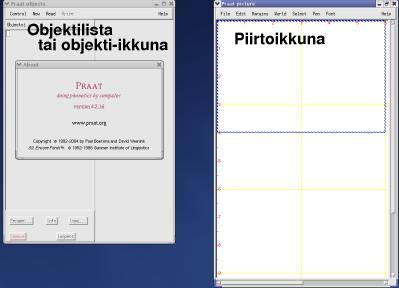
\includegraphics{/home/lennes/praat-opas/kuvat/kaynnistyskuva.jpg}


\caption{\label{fig:kaynnistys}Praat-ohjelma käynnistyy.}
\end{figure}



\subsection{Praat-ohjelman päivitykset}

Praat-ohjelmaan tulee uusia päivityksiä jopa kerran tai kahdesti kuukaudessa.
Yleensä päivityksen myötä saadaan käyttöön uusia toimintoja tai korjataan
edellisten ohjelmaversioiden vikoja. Joskus harvoin valikkokomennot
tai niiden sijainti voivat vähän muuttua ohjelmaversiosta toiseen.
Kovin laajoja muutoksia Praatin käyttöön ei tehdä, ja pienempiäkin
muutoksia toteutetaan yleensä vain useiden käyttäjien hyvin perustellusta
toivomuksesta. Tavallisesti on hyvä päivittää oman koneensa ohjelmaversio
säännöllisesti uudempaan (ks. asennusohjeet kohdasta \ref{sec:Mista-Praat-ohjelman-saa?}).


\subsection{\label{sub:Objektilista}Objektilista}

Kaikki Praat-ohjelmassa käsiteltävä aineisto näkyy objekti-ikkunassa
(ks. kuva \ref{fig:objektilista}).


\subsubsection{\label{par:Objektien-valitseminen}Objektien valitseminen}

Objekti valitaan\index{objektin valitseminen}\index{objektin aktivointi}\index{aktivointi}\index{valitseminen}
(\emph{select}\index{select}) näpäyttämällä sitä kerran hiirellä,
jolloin aktivoitu l. valittu objekti tummenee (ks. kuva \ref{fig:objektilista}).

Useampia, listalla peräkkäisiä objekteja voit valita näpäyttämällä
ensin yhtä objektia hiirellä ja pitämällä sitten \emph{vaihtonäppäimen}
(\emph{Shift}) pohjassa, kun näpäytät toista objektia.

Jos haluat valita useampia objekteja niin, että peräkkäisten objektien
välille jää ei-aktiivisia objekteja, pidä \emph{Control}-näppäin pohjassa
ja napsauttele samalla yksittäisiä objekteja. Toistuva näpäyttely
Control-näppäimen kanssa kytkee objektin vuorotellen aktiiviseksi
ja ei-aktiiviseksi.%
\begin{figure}
\includegraphics{/home/lennes/praat-opas/kuvat/objektit.jpg}


\caption{\label{fig:objektilista}Objektilistassa olevia objekteja voi valita
eli aktivoida hiirellä. Objektin kohdalla lukee ensin objektin tyyppi
(esim. Sound tai Pitch) ja sen jälkeen objektin nimi, jota käyttäjä
voi muuttaa. Objekti-ikkunan oikeassa reunassa olevan dynaamisen valikon
sisältö muuttuu sen mukaan, minkä tyyppinen objekti on valittuna.}
\end{figure}



\subsubsection{Objektien hallintapainikkeet}

Objektilistan alareunassa on lisäksi muutama painike. \textbf{Copy\ldots{}}
\index{objektin kopioiminen}-painikkeella voit tehdä kopion listalta
valitusta objektista (komento kysyy nimen uudelle objektille). \textbf{Info}\index{objektin tiedot}-painike
näyttää joitakin tietoja aktiivisesta objektista.

Alimpana ja punaisella näkyy \textbf{Remove}\index{objektin poistaminen objektilistasta}-painike,
joka \textbf{\emph{poistaa kaikki sillä hetkellä valittuna olevat
objektit mitään kyselemättä.}} Ole siis varovainen tämän painikkeen
kanssa, sillä jos et ole tallentanut poistettavia objekteja, ne häviävät
iäksi!


\subsubsection{\label{par:Kiintea-valikko-objektilistassa}Kiinteä valikko (fixed
menu)}

Objektilistaan liittyvä kiinteä valikko\index{kiinte\"a valikko objektilistassa}
näkyy objektilistan yläreunassa (tai Macissa näytön yläreunan valikkopalkissa,
ks. Mac-ohjeita esim.\citet{Lennes}).


\subsubsection{\label{par:Dynaaminen-valikko-(dynamic}Dynaaminen valikko (dynamic
menu)}

Dynaamisen valikon\index{dynaaminen valikko} sisältö muuttuu sen
mukaan, minkä tyyppinen objekti on valittuna (aktiivisena\index{aktiivinen objekti},
tummennettuna) objektilistassa. Jos listassa ei ole yhtään objektia
tai mikään objekteista ei ole valittuna, dynaamisen valikon alue on
kokonaan tyhjä.


\subsection{\label{sub:Piirtoikkuna}Piirtoikkuna}

Piirtoikkunaa\index{piirtoikkuna}\index{Picture-ikkuna} tarvitaan
silloin, kun halutaan piirtää Praatilla kuvia siirrettäväksi muihin
ohjelmiin. Piirtoikkunaan tehty kuva voidaan tallentaa esimerkiksi
korkealaatuisena EPS-grafiikkatiedostona tai se voidaan siirtää piirtoikkunasta
leikepöydälle ja ''liimata'' sellaisenaan vaikkapa tekstinkäsittelydokumenttiin.
Praatilla voidaan piirtää kuvia erilaisista akustisista analyyseista
tai numeerisesta datasta.

Kuvan piirtäminen tapahtuu periaatteessa aina jonkin objektilistaan
(ks. \ref{sub:Objektilista}) luodun objektin pohjalta: valitse objektilistasta
objekti, josta kuva piirretään, ja valitse dynaamisesta valikosta
(\ref{par:Dynaaminen-valikko-(dynamic}) haluamasi Draw- tai Paint-komento.
Valitusta objektista riippuen tarjolla voi olla useita erilaisia Draw-komentoja.
Komennon tuottama kuva piirtyy ja skaalautuu piirtoikkunasta valittuna
olevan piirtoalueen (\emph{Viewport}) mukaisesti. Piirtoikkunan sisällä
kuvan koostamista voidaan jatkaa lisäämällä esim. tekstiä piirtoalueen
eri kohtiin. Lisää kuvin piirtämisestä kerrotaan luvussa \ref{sec:Kuvien-luominen}.


\section{Tiedostojen hallinta}


\subsection{\label{sub:Tiedostojen-avaaminen-Praatissa}Tiedostojen avaaminen
Praatissa}

Kaikki Praat-ohjelman tunnistamat tiedostomuodot avataan periaatteessa
samalla tavalla: valitsemalla objekti-ikkunan \textbf{Read}-valikosta
\textbf{Read from file...} Praatissa ei ole väliä sillä, mikä on avattavan
tiedoston nimen pääte, sillä ohjelma tunnistaa automaattisesti objektin
tyypin tiedostoa lukiessaan. (Ks. kuitenkin tiedostojen nimeämiskäytänteitä
kohdasta \ref{sub:Tiedostojen-nimeamistavat}.)

Poikkeuksena normaalista tiedostojen avaamiskäytännöstä ovat hyvin
pitkät äänitiedostot, jotka eivät ehkä mahdu tietokoneen muistiin
kerralla:


\subsubsection{Erittäin pitkät äänitiedostot\index{pitkät \"a\"anitiedostot} (LongSound\index{LongSound})}

\textbf{\label{sub:LongSound}}Erittäin pitkien äänitiedostojen avaamiseen
on olemassa erikseen varakomento \textbf{Open long sound file...}
Sitä käytettäessä äänitiedosto aukeaa objektilistaan \textbf{LongSound}-tyyppisenä.
LongSound-objektina voidaan Praatissa käyttää jopa 3 GB:n kokoisia
äänitiedostoja. 

LongSound-objekteja voidaan selailla ja kuunnella LongSound-editorilla
samaan tapaan kuin Sound-objektejakin (vrt. äänieditori, \ref{sec:Aanieditori-(Sound-editor)}).
LongSound-objektin sisältämää äänisignaalia ei kuitenkaan lueta tietokoneen
käyttömuistiin kokonaisuudessaan, vaan muistissa pidetään ainoastaan
editorin näytöllä oleva osa. Tämän vuoksi LongSound-objektia ei voida
analysoida kokonaisena, eikä sille muutenkaan voida suorittaa aivan
samoja toimenpiteitä kuin Sound-objektille. LongSound-objektista voidaan
kuitenkin \textbf{Extract part...}-komennolla eristää pienempiä osia,
joita voidaan käsitellä tavallisina Sound-objekteina.


\subsection{\label{sub:Tiedostojen-tallentaminen-Praatissa}Tiedostojen tallentaminen
Praatissa}

\label{sub:Praatin-kayttamat-tiedostomuodot}Mikä tahansa Praat-ohjelmassa
käsiteltävänä oleva objekti voidaan tallentaa valitsemalla ensin kyseinen
objekti objektilistalta ja valitsemalla sen jälkeen sopiva tallennusvaihtoehto
objekti-ikkunan \textbf{Write}-valikosta.

Kaikki Praat-ohjelmassa käsitellyt objektityypit voidaan tallentaa
Write-valikon kautta joko tekstitiedostoina (\emph{text file}), lyhyinä
tekstitiedostoina (\emph{short text file}) tai binääritiedostoina
(\emph{binary file}). Monia analyysiobjekteja (esim. Pitch-objektit)
voidaan tallentaa pelkästään näihin kolmeen tiedostomuotoon. Sen sijaan
esimerkiksi ääniobjektit (Sound) voidaan lisäksi tallentaa useisiin
äänitiedostoformaatteihin (AIFF, WAV jne., ks. \ref{sec:aanitiedostoformaatit})
ja jotkut taulukon kaltaiset objektit (esim. TableOfReal) voidaan
tallentaa raakatekstitiedostoon, jossa kunkin taulukon rivin sarakkeet
on erotettu toisistaan sarkainmerkeillä. Viimeksimainittu muoto on
kätevä, jos Praatilla käsiteltyjä taulukoita halutaan siirtää esimerkiksi
Exceliin tai muihin taulukko- ja tilastolaskentaohjelmiin.


\subsubsection{\label{sub:Tiedostojen-nimeamistavat}Tiedostojen nimeämiskäytänteitä}

Vaikka Praat-ohjelmaa käyttäessä tiedostojen nimillä ei periaatteessa
ole väliä, on hyvä noudattaa tiettyä käytäntöä, jotteivät erityyppiset
tiedostot menisi sekaisin. Praatissahan voi luoda esimerkiksi ääniobjektista
monta analyysiobjektia, jotka ovat oletusarvoisesti samannimisiä kuin
ääniobjekti, josta ne tehtiin. Identtinen tiedostonimen alkuosa on
hyödyllinen, jos pitää jälkeenpäin tunnistaa, mikä analyysitiedosto
vastaa mitäkin äänitiedostoa. Tätä voi hyödyntää etenkin skriptauksessa
(\ref{cha:Skriptaus}). 

Tiedostonimille on tapana antaa pisteellä erotettu pääte tiedoston
tyypin mukaan. Esimerkiksi äänitiedostojen nimi päättyy .wav, .aif
sen mukaan, missä ääniformaatissa ne tallennettiin. Äänitiedostosta
\emph{kukka.aif} tehty Pitch-objekti kannattaisi siis tallentaa nimellä
\emph{kukka.Pitch} ja formanttianalyysi nimellä \emph{kukka.Formant}.
Praat-skriptitiedostotkin ovat periaatteessa tavallisia tekstitiedostoja,
mutta ne kannattaisi tallentaa vastaavilla tunnisteilla, esimerkiksi
\emph{omaSkripti.praat}, jolloin jo tiedoston nimestä näkee, ettei
kyseessä ole mikä tahansa teksti.


\chapter{\label{sec:Aanieditori-(Sound-editor)}Äänieditori (Sound editor)}

Äänieditori on Praatin ikkuna, jossa voidaan selailla tiettyä ääniobjektia,
kuunnella siitä eripituisia pätkiä ja katsella samalla äänen aaltomuotoa
sekä äänestä laskettuja erilaisia akustisia analyyseja. 


\section{\label{sub:Aanen-kuuntelu}Äänen kuuntelu}

Objektilistalta valitun ääniobjektin voi kuunnella 

\begin{itemize}
\item kokonaisuudessaan painamalla sen viereisestä dynaamisesta valikosta
painiketta \textbf{Play}. Jos ääniobjekti on huikean pitkä ja haluatkin
keskeyttää kuuntelun, paina Esc-näppäintä.
\item pienemmissä pätkissä avaamalla äänieditori-ikkunan:
\end{itemize}

\section{\label{sec:Aanieditorin-kaytto}Äänieditorin käyttö}

Äänieditorin käyttämiseksi äänitiedosto on ensin avattava Praatin
objektilistaan (\textbf{Read: Read from file...}). Kun haluttu ääniobjekti
on objektilistalla aktiivisena, paina objektilistan oikeassa laidassa
näkyvästä dynaamisesta valikosta painiketta \textbf{Edit}, jolloin
äänieditori avautuu. Editori-ikkunoita voi olla samanaikaisesti avoinna
useita myös samasta ääniobjektista.

Äänieditorin yläosassa näkyy äänen aaltomuoto mustana käyränä%
\footnote{Aaltomuodon päällä voi myös näkyä sinisiä pystyviivoja (Pulses), jotka
liittyvät perustaajuusanalyysiin. Pulssit voi kytkeä pois päältäkin,
sillä yleensä niitä ei tarvita, ja ne vain sekoittavat aaltomuotokuvaajaa.
Pulssien näkymistä voi vaihtaa valitsemalla äänieditori-ikkunan \textbf{Pulses}-valikosta
\textbf{Show pulses}.%
}. 

\begin{description}
\item [aaltomuoto\index{aaltomuoto}~(waveform\index{waveform})]Äänen
aaltomuodolla tarkoitetaan äänisignaalista piirrettyä kuvaa, jossa
alkuperäisestä äänestä mikrofonilla mitatut ilmanpaineen vaihtelut
näkyvät aaltomaisena käyränä. Koska mikrofoni on oikeastaan muuntanut
ilmanpaineen sähköksi eli jännitemuutoksiksi ja tämä prosessi riippuu
myös mikrofonin ominaisuuksista, alkuperäistä ilmanpainetta ei kuitenkaan
voida kuvasta nähdä. Aaltomuotokuvassa aika etenee vasemmalta oikealle.
Pystyakseli kuvaa tietyin väliajoin mikrofonin keräämästä sähköisestä
signaalista rekisteröityjä arvoja. 
\end{description}
%
\begin{figure}
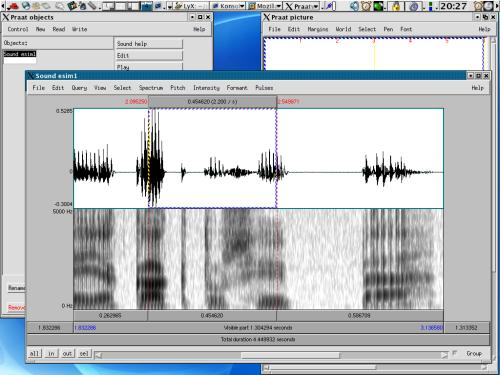
\includegraphics[%
  scale=0.8]{/home/lennes/praat-opas/kuvat/aanieditori.jpg}


\caption{Tältä näyttää Praat-ohjelman äänieditori-ikkuna (Sound Editor), jossa
voi kuunnella äänen eri kohtia ja tehdä siitä pieniä mittauksiakin.}
\end{figure}



\subsection{\label{sub:Aanen-patkien-kuuntelu-editorissa}Äänen pätkien kuuntelu}

Äänieditorin alalaidassa näkyy 2--3 tummanharmaata \textbf{soittopalkkia}.
Palkkien avulla voidaan kuunnella äänestä eri pätkiä. Kun napsautat
hiirellä alinta palkkia, kuulet koko ääniobjektin yhtä soittoa. Toiseksi
alimmaisesta palkista voit soittaa äänestä tällä hetkellä näkyvissä
olevan alueen. Jos maalaat hiirellä lyhyemmän, laatikkomaisen alueen
keskeltä aaltomuoto- tai analyysikuvia, voit käyttää kolmatta, ylimmäistä
soittopalkkia, joka ''katkeaa'' valitun alueen rajoilta. Näin voit
soittaa kerralla haluamasi pätkän, tai pätkän sitä ennen, tai pätkän
heti sen jälkeen. 

Kunkin soittopalkin keskellä lukee kyseisen palkin kuvaaman ajanjakson
kesto sekunteina: alimmassa palkissa koko ääniobjektin kesto (\emph{Total
duration}), keskimmäisessä palkissa näkyvissä olevan alueen kesto
(\emph{Visible part}), ja ylimmässä lyhyempien pätkien kestot hiirellä
valitsemasi alueen mukaisesti. 


\section{\label{sub:Aanen-muokkaaminen-(leikkaa-liimaa-toiminnot)}Äänen muokkaaminen
(leikkaa-liimaa-toiminnot)}

Tätä osiota ei ole vielä kirjoitettu.


\section{\label{sec:Analyysikuvaajat-editorissa}Analyysikuvaajat äänieditorissa}

Jos äänestä on valittu näkyviin analyyseja, kuten spektrogrammi (Spectrogram;
näkyy harmaasävyinä), F0-käyrä (Pitch; sinisellä), intensiteettikäyrä
(Intensity; keltaisella) tai formanttianalyysi (Formant; punaiset
pisteet), nämä näkyvät äänieditorin alaosassa päällekkäin. Analyysikuvaajat
voidaan kytkeä päälle tai pois valitsemalla äänieditori-ikkunan valikoista
\textbf{Spectrum: Show spectrogram}, \textbf{Pitch:Show pitch}, \textbf{Intensity:Show
intensity} tai \textbf{Formant:Show formants}. 

Esimerkiksi formanttianalyysin pitäminen näkyvissä hidastaa äänieditorin
käyttöä, sillä aina ikkunan näkymän muuttuessa kone laskee analyysit
uudelleen. Analyysit kannattaa siis kytkeä pois päältä kun niitä ei
välttämättä tarvita.


\subsection{\label{sec:Mittausten-tekeminen-aanieditorissa}Mittausten tekeminen
äänieditorissa}

Äänieditorissa näkyvistä analyysikuvista voi tehdä yksittäisiä numeerisia
mittauksia hiiren avulla. Laajempi aineisto kannattaa ensin nimikoida
(ks. \ref{sec:Nimikointi}), jotta mitattavat kohdat löytyvät helposti
ja mittaukset ovat tarvittaessa toistettavissa. Nimikoidusta aineistosta
on myös mahdollista tehdä mittauksia täysin automaattisesti skriptien
(\ref{cha:Skriptaus}) avulla.


\subsubsection{\label{sub:Kestot-aanieditorissa}Kestot\index{kestomittaukset}}

Voit tehdä äänieditorissa suurpiirteisiä kestomittauksia valitsemalla
äänestä mitattavan pätkän, esimerkiksi tietyn äänteen tai sanan, ja
katsomalla valitun alueen keston ylimmästä soittopalkista. Keston
saa myös näkyviin valitsemalla \textbf{Query:Get selection length},
jolloin tarkka arvo ilmestyy ns. Info-ikkunaan ja sen voi vaikkapa
kopioida hiirellä toiseen ohjelmaan. Sama mittausmenetelmä toimii
myös TextGrid-editorissa. Alueiden valinta yksi kerrallaan käsin on
työläs tapa mitata kestoja, ja laajemman aineiston mittauksia varten
aineisto kannattaakin nimikoida etukäteen (ks. \ref{sec:Nimikointi})
ja käyttää mahdollisesti skriptiä nimikoitujen pätkien kestomittauksiin.


\subsubsection{Spektrogrammi, perustaajuus, intensiteetti ja formantit}

Kun valitset äänieditoriin näkyviin erilaisia analyysikuvia, voit
tehdä niistä mittauksia hiiren avulla. Klikkaa haluamaasi kohtaan
analyysikuvassa. Näkyviin tulee punainen ristikko eli kursori. Pystyviivan
kohdalla oleva mitattava aikapiste näkyy pystyviivan yläpäässä. 

Jos haluat tämän aikapisteen kohdalta tietoa spektrogrammista (\ref{sub:Spektrogrammi}),
näet editorin vasemmassa laidassa punaisen numeron, joka ilmoittaa
spektrogrammissa näkyvän taajuuden kursorin \emph{vaakaviivan} kohdalla.
Spektrogrammin pystyakselihan vastaa taajuutta. Samassa kohtaa näkyy
myös formanttitaajuus, jos kursorin ristikko on tarkalleen jonkin
punaisen formanttipisteen päällä. Mikäli näkyvissä on sininen \emph{Pitch}-
eli perustaajuuskäyrä, näkyy punaisen pystykursorin kohdalta mitattu
perustaajuus sinisellä oikeassa laidassa (huom. älä sekoita tätä spektrogrammimittaukseen,
joka näkyy vasemmalla!). Intensiteetti näkyy myös oikeassa laidassa,
mutta analyysikuvan sisäreunassa ja vihreillä numeroilla. Kaikki nämä
lukuarvot saat tarvittaessa poimituksi tarkasti Info-ikkunaan valitsemalla
ko. analyysin valikosta vastaavan \textbf{Get}-komennon. Esimerkiksi
perustaajuuskäyrän arvon saat \textbf{Pitch}-valikon komennolla \textbf{Get
pitch}. 

Lisää akustisista analyyseista kerrotaan luvussa \ref{sec:Akustinen-analyysi}.


\chapter{\label{sec:Nimikointi}Nimikointi }

\emph{Nimikoinnilla}\index{nimikointi} (engl. \emph{labeling}\index{labeling})
eli \emph{annotoinnilla} (\emph{annotation, to annotate}\index{annotation})
tarkoitetaan sitä, että (digitaalisesti) tallennettuun puhenäytteeseen
liitetään systemaattisesti \emph{annotaatioita\index{annotaatio}}
(\emph{annotation}\index{annotation}) eli jonkinlaisia (symbolisia)
kuvauksia näytteen sisällöstä. Nimikointi tehdään yleensä jollakin
tähän tarkoitukseen kehitetyllä tietokoneohjelmalla, joista Praat
on yksi vaihtoehto. Ääninäytteen on oltava digitaalisessa muodossa
ts. äänitiedostona esim. tietokoneen kovalevyllä tai jonkintyyppisillä
levykkeillä. Ääninäytettä kuunnellaan ja siitä piirrettyjä kuvia katsellaan
analyysiohjelmalla. Kuuntelun ja katselun perusteella kirjoitetaan
ääninäytteen ''pariksi'' \emph{nimikointitiedosto}\index{nimikointitiedosto},
joka sisältää ääninäytteen kuvaukset. Nimikoinnin tarkoituksena on
muodostaa \char`\"{}maamerkkejä\char`\"{}, joiden perusteella alkuperäisestä
puhesignaalista voidaan löytää halutut osat ja kohdistaa niihin vaikkapa
akustisia analyyseja tai muita toimenpiteitä. Nimikointi on välttämätöntä,
jos halutaan hallita ja hyödyntää suurta määrää puheaineistoa.

\textbf{Nimikoinnissa annotaatiot on sidottava ääninäytteen aikaulottuvuuteen.}
Tätä varten ääninäyte yleensä \emph{segmentoidaan}\index{segmentoida}:
siitä rajataan halutulla tarkkuudella \emph{segmenttejä\index{segmentti}}
(äänipätkiä, joilla on määrätty alku- ja loppupiste sekä ajallinen
kesto; engl. \emph{segment}\index{segment}). Segmenteille voidaan
sitten antaa nimiä eli \emph{nimikoida} ne. Myös ääninäytteen tietyille
yksittäisille ajanhetkille (aikapisteille) voidaan antaa nimiä (näin
syntyy ns. \emph{ankkureita}\index{ankkuri}, \emph{}engl. \emph{point}\index{point}).
Pelkkä ääninäytteen litterointi esimerkiksi tekstitiedostoon ei siis
ole nimikoimista, koska siinä litteraation eri osia ei kytketä ääninäytteen
vastaaviin ajallisiin kohtiin.%
\footnote{Kannattaa huomata, että litteraatio tai mikä tahansa muu transkriptio
on aina \emph{tulkinta} alkuperäisestä aineistosta. Siksi \emph{pelkän}
litteraation avulla ei pitäisi koskaan tutkia \emph{puhetta} --- vaarana
on, että tulee pikemminkin tutkineeksi litteroijan näkemystä, joka
on vieläpä kuvattu \emph{kirjoitetulla} kielellä! Käyttämällä nimikointia
aineiston kuvausmenetelmänä varmistetaan mahdollisimman suora yhteys
alkuperäiseen puhetallenteeseen, jolloin tutkijalla ja tutkimuksen
arvioijalla on mahdollisuus tarkistaa ja korjailla puheesta luotuja
kuvauksia.%
}

Annotaatiotyylejä on erilaisia ja tutkija voi kehittää oman annotaatiotavan
sen mukaan, minkälaisista puheen ilmiöistä on kiinnostunut. Annotaatio\index{annotaatio}
voi olla esimerkiksi ortografinen ts. oikeinkirjoitusta noudattava
litteraatio\index{litteraatio} (engl. yl.~\emph{transliteration}\index{transliteration},
\emph{transcript}\index{transcript}), morfologisten yksiköiden kuvaus,
prosodisten piirteiden kuvaus tai vaikkapa foneettinen \emph{transkriptio}\index{transkriptio}\index{foneettinen transkriptio}
(engl. \emph{transcription}) puheesta. Ensin mainitussa tapauksessa
segmenttirajat voivat olla vaikkapa yksittäisten sanojen tai lauseiden
välillä, kun taas foneettista tutkimusta varten rajataan usein yksittäisiä
äänteitä.

Jos erilaisia puheen yksiköitä halutaan käyttää hyödyksi yhdessä,
voidaan luoda useita annotaatio- tai nimikointikerroksia\index{nimikointikerros}
tai -tasoja: yhdelle merkitään äänteiden rajat, toiselle sanojen rajat,
kolmannelle lauserajat jne.

Automaattisia segmentointi\index{automaattinen segmentointi}- ja
nimikointimenetelmiä yritetään jatkuvasti kehittää eri puolilla maailmaa.
Toistaiseksi tarkimman nimikoinnin saa kuitenkin aikaan ihminen, sillä
puheen nimikointi vaatii monenlaisten kielellisten tulkintojen tekemistä.
Samasta syystä voidaan valitettavasti todeta myös, että sekä puheen
litterointi, transkriptio että nimikointi ovat aina jossakin määrin
subjektiivisia tuotoksia: niiden tarkkuus ja johdonmukaisuus riippuvat
nimikoijan intresseistä, tiedoista, taidoista ja teoreettisesta näkemyksestä.


\section{Miksi puhetta nimikoidaan eli annotoidaan?}

\begin{itemize}
\item Nimikointityökalua käyttämällä puhenäytteestä on helppo nopeasti ja
tarkasti etsiä, rajata ja kuunnella eri pituisia osia. Tämä helpottaa,
nopeuttaa ja tarkentaa merkittävästi litterointia ja transkriptiota.
Esimerkiksi intonaatiotranskription\index{intonaatiotranskriptio}
tekeminen helpottuu, kun kuulohavaintoa voidaan heti verrata äänisignaalista
laskettuun perustaajuuskäyrään.
\item Nimikoidusta äänitiedostosta voidaan mitata tarkasti puheen eri yksiköiden
kestoja. Mittauksia voidaan suorittaa jopa täysin automaattisesti
(edellyttäen että puhe on nimikoitu mittausten kannalta järkeviin
yksiköihin). Akustiset analyysit voidaan kohdistaa vain tarvittaviin
osiin näytettä. 
\item Nimikoinnin perusteella tehdyt mittaukset voidaan milloin tahansa
toistaa täysin identtisinä. Tutkimustuloksiin on siten helppo myöhemmin
palata. 
\item Alkuperäistä digitoitua ääninäytettä (esim. keskusteluäänite) ei tarvitse
välttämättä pilkkoa pienempiin osiin jokaista tutkimusta tai demoa
varten, vaan se voidaan säilyttää kokonaisena esimerkiksi CD-ROMilla,
eikä tällöin menetetä informaatiota esimerkiksi taukojen kestoista. 
\item Digitaalinen ääninäyte säilyy tarvittaessa täysin muuttumattomana
pitkiäkin aikoja ja siitä voidaan tehdä identtisiä kopioita. 
\item Digitaalisia ääni- ja nimikointitiedostoja on helppo jakaa muidenkin
tutkijoiden kanssa. Muut tutkijat voivat nopeasti tutustua nimikoituun
puhenäytteeseen ja käyttää sitä. Nimikointiin voidaan tehdä muutoksia
ja lisäyksiä oman tarpeen mukaan. 
\item Nimikoitu äänitiedosto voidaan lopulta liittää osaksi kaikkien tutkijoiden
käyttämää puhetietokantaa , eikä tutkijoiden tarvitse aina itse kerätä
ja nimikoida uusia aineistoja.
\end{itemize}

\section{\label{sub:Praat-ohjelmalle-tyypillisia-nimikointiominaisuuksia}Praat-ohjelmalle
tyypillisiä nimikointiominaisuuksia}

\begin{itemize}
\item mahdollisuus tehdä useita nimikointikerroksia (\emph{tiers}), ts.
voidaan kuvata samanaikaisia mutta eri tyyppisiä tapahtumia useilla
eri tasoilla 
\item mahdollisuus lisätä segmenttien (\emph{intervals}) lisäksi myös nimettyjä
aikapisteitä (\textbf{PointTier}-tyyppisille riveille)
\item nimikointitiedostojen (TextGrid) ja äänitiedostojen erillisyys, ts.
äänitiedostoa ei nimikoitaessa muuteta - vain nimikointitiedosto muuttuu
\item mahdollisuus nimikoida erittäin pitkiä äänitiedostoja yhtenäisinä
(LongSound-objekteina voidaan avata jopa useiden tuntien kestoisia
ääninäytteitä esim. CD-ROMilta)
\item nimikointitiedostojen siirrettävyys laitteistosta ja ympäristöstä
toiseen (TextGridit voidaan tallentaa tavallisina tekstitiedostoina)
\item mahdollisuus skriptien avulla kohdistaa akustinen yms. analyysi haluttuihin
kohtiin nimikoituja ääninäytteitä.
\end{itemize}

\section{Miten Praat-ohjelmalla nimikoidaan puhetta? }

Ennen kuin aloitat äänitiedoston nimikoinnin, varmista, että ääni
on juuri sen mittainen ja editoitu sellaiseksi kuin haluat. Nimikointia
varten luodaan nimittäin \emph{TextGrid-objekti}\index{TextGrid-objekti},
jonka on oltava \textbf{samankestoinen kuin sitä vastaava äänitiedosto}.
Jos äänitiedoston kesto myöhemmin muuttuu (esim. päätät poistaa sen
alusta \char`\"{}turhaa tyhjää\char`\"{}) ja olet jo aloittanut nimikoinnin,
joudut vaikeuksiin, koska TextGridiin merkitsemäsi segmenttirajat
eivät enää vastaakaan alkuperäisiä aikapisteitä äänisignaalissa. Onkin
sitten hankalampi juttu siirtää segmenttirajat taas oikeisiin paikkoihin\ldots{}


\subsection{\label{sub:Nimikointiobjektin-luominen-Praatissa}Nimikointiobjektin
luominen Praatissa}

\begin{enumerate}
\item Avaa objektilistaan haluamasi äänitiedosto joko Sound-objektina tai
LongSound-objektina \ref{sub:Tiedostojen-avaaminen-Praatissa}. Käytä
LongSound-objektityyppiä (komento \textbf{Read: Open long sound file...})
siinä tapauksessa, että äänitiedosto on erityisen suuri, eikä mahdu
kerralla tietokoneesi käyttömuistiin. Varmista, että ääniobjekti on
valittuna. 
\item Paina objektilistan oikeassa laidassa näkyvää painiketta \textbf{Annotate:
To TextGrid\ldots{}} Näkyviin tulee lomake (ks. kuva \ref{fig:textgridin_luonti}).
Kirjoita ylemmälle riville (\emph{Tier names}) välilyönneillä erotettuna
nimet niille nimikointikerroksille, joiden haluat olevan TextGrid-objektissa.
Jos kirjoitat vaikkapa \char`\"{}\emph{äänteet sanat lauseet}\char`\"{},
saat kolme nimikointikerrosta. Voit muuttaa, lisätä ja poistaa nimiä,
kerroksien määrää ja kerrostyyppejä myöhemminkin (ks. \ref{sub:Nimikointikerroksien-lis=E4=E4minen-ja}).
\item Oletuksena kaikki ylärivillä mainitut nimikointikerrokset luodaan
IntervalTier-tyyppisinä. IntervalTier-kerroksiin\index{IntervalTier}
voi nimikoida vain segmenttejä\index{segmentti}, eli aikavälejä joilla
on alku- ja loppuraja. Jos kuitenkin haluat, että jotkut nimikointikerroksista
ovat tyyppiä PointTier, kirjoita näiden nimet myös alemmalle riville
(Point tiers). PointTier-rivien nimien tulee siis esiintyä molemmissa
kohdissa. PointTier-kerroksiin\index{PointTier} voi merkitä yksittäisiä
aikapisteitä, joille voi antaa nimiä. Joskus tällaisistakin merkkipaaluista
voi olla iloa.
\item Paina OK. Objektilistaan ilmestyy uusi TextGrid-objekti, joka näkyy
valittuna. Nyt voit aloittaa varsinaisen nimikoinnin.%
\begin{figure}
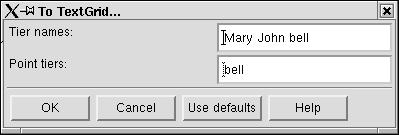
\includegraphics{/home/lennes/praat-opas/kuvat/textgridin_luonti.jpg}


\caption{\label{fig:textgridin_luonti}Tällä lomakkeella voidaan määrittää
uuden TextGrid-objektin nimikointikerrosten nimet ja tyypit. Ylemmälle
riville kirjoitetaan kaikkien kerrosten nimet. Jos haluat jonkin kerroksen
olevan tyyppiä PointTier (eikä IntervalTier), mainitse kerroksen nimi
myös lomakkeen alemmalla rivillä. Kerroksia ja niiden nimiä voi myös
muokata jälkeenpäin.}
\end{figure}

\end{enumerate}

\subsection{\label{sub:Nimikointi}Nimikointi}

\begin{enumerate}
\item Valitse objektilistasta samanaikaisesti ääniobjekti (Sound tai LongSound)
ja sitä vastaava TextGrid-objekti, jonka juuri loit. (Voit valita
kaksi objektia yhtä aikaa pitämällä Shift- eli vaihtonäppäintä tai
Control-näppäintä pohjassa, kun naksautat toista objektia.)
\item Paina oikealla näkyvää painiketta \textbf{Edit}. Uusi \emph{TextGrid-editori}\index{TextGrid-editori}\index{nimikointi-ikkuna}\index{annotaatioeditori}-ikkuna
avautuu. Ikkunan yläosaa hallitsee äänisignaalin kuvaus: Ylimpänä
näkyy äänen aaltomuoto\index{aaltomuoto} eli oskillogrammi, ja sen
alapuolella saattaa olla toinen ikkuna, jossa on äänestä laskettuja
analyysikuvia (esim. spektrogrammi, ks. \ref{sub:Spektrogrammi}).
Äänisignaalikuvien yläpuolella on kapea valkoinen osa, \emph{kirjoitustila}.
Ikkunan alareunassa näkyy valkoisia palkkeja: ne ovat \emph{}nimikointirivejä
eli \emph{nimikointikerroksia}\index{nimikointikerros} (\emph{tier}).
Aktiivisena oleva nimikointirivi näkyy keltaisena.
\item TextGrid-editorissa voit kuunnella ääntä ja sen pätkiä samalla tavalla
kuin Sound- ja LongSound-editoreissa (ks. luku \ref{sec:Aanieditori-(Sound-editor)}).
Editori-ikkunan alalaidassa (valkoisten nimikointikerrosten tai -rivien
alla) näkyy kaksi tai kolme vaakasuoraa palkkia. Kun painat alinta
palkkia, kuulet koko ääniobjektin sisällön yhtä soittoa. Toiseksi
alin palkki soittaa koko tällä hetkellä näkyvissä olevan osan äänestä
- voit käyttää tätä toimintoa, kun zoomaat äänikuvaa sisään- tai ulospäin
tai vierittelet kuvaa oikealle tai vasemmalle. Kolmesta soittopalkista
ylimmäinen tulee näkyviin, kun naksautat hiirellä johonkin kohtaan
ääniaaltoa tai analyysikuvaa tai kun valitset äänestä alueen vetämällä
hiirellä sen yli. Ylimmällä soittopalkilla voit kuunnella äänestä
minkä tahansa lyhyenkin pätkän, kun muutat välillä kursorin paikkaa
tai valitun alueen sijaintia. Kokeile!
\item Kun olet kuuntelemalla ja/tai katselemalla löytänyt kohdan (esim.
lauseen alku), johon haluat tehdä segmenttirajan, naksauta ensin hiirellä
kyseiseen kohtaan ääniaaltoa tai analyysikuvaa ikkunan yläosassa.
Alaosan valkoisiin nimikointikerroksiin (\emph{tiers}) ilmestyy pystyviiva,
jossa on pieni ympyrä jokaisen nimikointikerroksen yläreunassa. Naksauta
hiirellä tarkasti ympyrään sen nimikointikerroksen kohdalle, johon
haluat lisätä segmenttirajan. Uusi raja tulee näkyviin paksuna pystyviivana.
%
\begin{figure}
\includegraphics{/home/lennes/praat-opas/kuvat/add_boundary.jpg}


\caption{Kun haluat lisätä johonkin annotaatiokerrokseen uuden rajan, klikkaa
ensin hiirellä oikeaa kohtaa aaltomuodosta tai analyysikuvasta, ja
klikkaa sitten pientä ympyrää haluamasi nimikointikerroksen yläreunassa.}
\end{figure}


\begin{itemize}
\item Valittuna oleva segmenttiraja näkyy punaisena ja muut rajat sinisinä.
Tietyn rajan voi valita naksauttamalla hiirellä sen päällä.
\item Segmenttirajaa voi siirtää oikealle tai vasemmalle tarttumalla siihen
hiirellä (mutta ei viereisten segmenttirajojen yli). Kahta tai useampaa
eri nimikointikerroksissa mutta täsmälleen samassa aikapisteessä olevaa
segmenttirajaa voit siirtää yhtä aikaa pitämällä Shift- eli vaihtonäppäintä
pohjassa ja vetämällä yhtä rajoista.
\item Valitun (punaisen) segmenttirajan voi poistaa valitsemalla editori-ikkunan
\textbf{Point/Boundary}-valikosta \textbf{Remove}.
\item Jos haluat, että segmenttirajat ovat varmasti täsmälleen samassa aikapisteessä
useammassa nimikointikerroksessa, tartu yhteen rajaan ja vedä se hiirellä
toisessa kerroksessa olevan rajan päälle. Tällöin rajat menevät automaattisesti
samaan aikapisteeseen. (Tätä mahdollisuutta kannattaa käyttää hyväksi,
sillä silmämääräisesti rajoja on vaikea saada täsmälleen samaan kohtaan!)
\item Valittuna olevan nimikointikerroksen nimi näkyy punaisella tekstillä
TextGrid-editorin oikeassa reunassa ja kerroksen numero myös punaisella
vasemmassa reunassa.
\end{itemize}
\item Kun lause, äänne tms. yksikkö on rajattu ja haluat antaa segmentille
nimen, naksauta hiirellä haluamallesi nimikointikerrokseen niiden
rajojen väliin, johon haluat kirjoittaa. Kirjoita sitten segmentin
nimi tavalliseen tapaan näppäimistöllä. Teksti tulee samanaikaisesti
näkyviin nimikointikerrokseen segmentin kohdalle ja ikkunan yläreunassa
olevaan valkeaan \emph{kirjoitustilaan}\index{kirjoitustila}. (Huom.
Joissakin tapauksissa joudut ensin naksauttamaan ikkunan yläreunan
kirjoitustilaa, ennen kuin pääset kirjoittamaan tekstiä segmenttiin.)
Jo kirjoitettua tekstiä voit muokata normaalisti naksauttamalla ensin
ko. segmenttiä nimikointikerroksessa ja sitten haluttua tekstikohtaa
ikkunan yläosan kirjoitusrivillä.
\end{enumerate}

\subsubsection{\label{sub:nimikointivihjeita}Vihjeitä}

\begin{itemize}
\item Huomaa, että puheessa sanojen ja äänteiden välissä ei normaalitapauksessa
ole taukoja, joten seuraava äänne tai sana alkaa yleensä siitä mihin
edellinen loppuu!
\item On myös olemassa puheäänteitä, joiden keskellä on luonnostaan lyhyt
täysin hiljainen vaihe (esimerkiksi soinnittomat klusiilit {[}kpt{]}).
Tämä vaihe on osa äännettä (ja sanaa) eikä se ole siis varsinainen
tauko. Jos soinniton klusiili on puhunnoksen alussa ja sitä edeltää
tauko, et voi yleensä mitenkään päätellä, mistä kohtaa klusiilin sulkeumavaihe
on alkanut. Tässä tapauksessa kannattaa rajata ko. äänteeseen mukaan
pelkkä laukeamavaihe, josta syntynyt pieni ''pyrskähtävä'' ääni
on monesti nähtävissä aaltomuodossa aivan puhunnoksen alussa.
\item Puheen aikana ihmisen ääntöelimistö on lähes jatkuvassa liikkeessä.
Ei siis ole mikään ihme, että äännerajojen löytäminen vaatii kärsivällisyyttä
ja kompromisseja!
\item Jos joudut nimikoimaan paljon, kannattaa jo ergonomisista syistä opetella
muutama TextGrid-editorin valikkokomentoihin liittyvä näppäinoikotie,
jolla voit säästää paljon hiiren liikkeitä ja naksauttelua. Näppäinoikotiet
näkyvät Praatin valikoissa kyseisen komennon perässä. Esimerkiksi
rivinvaihtonäppäintä painamalla voit lisätä segmenttirajan valittuun
kerrokseen kursorin kohdalle (vrt. \textbf{Boundary}-valikon \textbf{Add
on selected tier}), eikä tarvitse osua hiirellä pieneen rinkulaan.
Sarkainnäppäimen (vastakkaiset nuolet näppäimistön vasemmassa yläreunassa)
painallus soittaa valitun äänipätkän. Ctrl-näppäin ja nuoli oikealle
aiheuttavat puolestaan siirtymisen seuraavaan segmenttiin valitussa
nimikointikerroksessa (vrt. \textbf{View}-valikon komento \textbf{Select
next interval}).
\item Valitun annotaatiokerroksen nimikkeistä voi etsiä tekstiä \textbf{Edit}-valikon
\textbf{Find\ldots{}}-komennolla. Toiminnosta on hyötyä, kun annotoit
pitkiä äänitiedostoja.
\end{itemize}

\subsection{\label{sub:Nimikointikerroksien-lis=E4=E4minen-ja}Nimikointikerroksien
lisääminen ja poistaminen}

TextGrid-editorin sisällä voit luoda lisää nimikointi- eli annotaatiokerroksia
ja kopioida tai poistaa olemassaolevia.

\begin{itemize}
\item Jos haluat lisätä editoitavaan TextGridiin uuden IntervalTier-tyyppisen
annotaatiokerroksen johon merkitään segmenttejä, valitse \textbf{Tier}-valikosta
\textbf{Add interval tier\ldots{}} Jos taas haluat luoda PointTier-tyyppisen
kerroksen, johon merkitään yksittäisiä nimettyjä aikapisteitä, valitse
\textbf{Add point tier\ldots{}}

\begin{itemize}
\item Näkyviin tulee lomake (ks. kuva \ref{cap:add_interval_tier}): Merkitse
\emph{Position}-kohtaan, monesko ylhäältä laskettuna uuden kerroksen
pitäisi annotaatiokerrosten ''pinossa'' olla (oletuksena uusi kerros
luodaan alimmaiseksi). Kirjoita luotavalle kerrokselle jokin kuvaava
nimi kohtaan \emph{Name}. Paina OK. Uusi kerros tulee heti näkyviin.
\end{itemize}
\end{itemize}
%
\begin{figure}
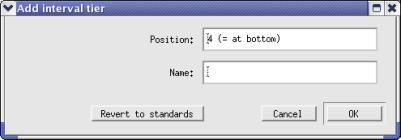
\includegraphics{/home/lennes/praat-opas/kuvat/add_interval_tier.jpg}


\caption{\label{cap:add_interval_tier}Anna uudelle annotaatiokerrokselle
paikka TextGridin kerrosten joukossa sekä jokin kuvaava nimi.}
\end{figure}


\begin{itemize}
\item Jos haluat poistaa TextGrid-objektista jonkin annotaatiokerroksen\index{annotaatiokerroksen poistaminen}
kaikkine merkintöineen, valitse ensin poistettava kerros klikkaamalla
hiirellä johonkin ko. kerroksen kohtaan. Varmista vielä, että oikea
kerros on valittuna ja sen numero ja nimi näkyvät punaisina TextGrid-editorin
laidoissa. Valitse sitten \textbf{Tier}-valikosta \textbf{Remove entire
tier}. Ole varovainen: tähän ei kysytä varmistusta, ennen kuin annotaatiokerros
katoaa! \textbf{Edit}-valikon \textbf{Undo}-komento saattaa tosin
pelastaa sinut vahingon sattuessa.
\item Jos haluat poistaa TextGridin tietyltä annotaatiokerrokselta kaiken
tekstin, toimi samoin kuin edellisessä kohdassa, mutta valitse komento
\textbf{Remove all text from tier}. Tällöin segmenttien rajat tai
ankkurit pysyvät paikoillaan, vain niiden nimikkeet hävitetään.
\item \label{ite:duplicate_tier}Voit kopioida tietyn annotaatiokerroksen
komennolla \textbf{Tier:Duplicate tier}. Tällöin sinulta kysytään
samat tiedot kuin luodessasi kokonaan uutta kerrosta (ks. kuva \ref{cap:add_interval_tier}).%
\footnote{Duplicate-komennolla voit jakaa esimerkiksi saman yksikön kaksi piirrettä
eri kerroksiin: annotoi ensin yksi piirrekerros, kopioi se, poista
kopiosta kaikki teksti ja nimikoi toinen piirrekerros.%
} 
\end{itemize}

\subsection{\label{sub:IPA-merkit-ja-erikoismerkit}IPA-merkit ja erikoismerkit}

Praatissa on oma tapa, jolla saa erikoismerkkejä näkyviin TextGridissä.
Erikoismerkit tuotetaan näppäilemällä peräkkäin \textbackslash{}-merkki
ja jotain muita merkkejä. Näin muodostetut merkit näkyvät siis ainoastaan
Praatin TextGrid-ikkunoissa ja piirtoikkunassa.%
\footnote{Jos et saa foneettisia merkkejä näkymään, joudut luultavasti ensin
asentamaan koneellesi erikseen ilmaisen \emph{SIL Doulos IPA}-kirjasimen,
jonka voit ladata verkosta. Linkki löytyy Praat-ohjelman kotisivulta
samasta kohdasta, josta hait myös Praat-ohjelman Windows-version.%
}

Kaikkien Praatissa näkyvien erikoismerkkien\index{erikoismerkit}
ja IPA-symbolien\index{IPA-symbolit}\index{foneettiset merkit} koodit
näet Praatin sisäisestä manuaalista: Kun olet TextGrid-editori-ikkunassa,
valitse sen oikeasta ylänurkasta \textbf{Help:About~special~symbols}.
Sivu on hiukan suttuinen, mutta kaikkien merkkikoodien pitäisi löytyä.
Voit myös yrittää käyttää manuaalin hakua (\textbf{Search~manual})
ja antaa hakusanaksi \char`\"{}symbols\char`\"{} tms. (ks. manuaalin
käyttö, \ref{sub:Praatin-sisaanrakennettu-manuaali}).

Esimerkiksi nuoli ylöspäin\index{nuoli ylöspäin} syntyy näppäilemällä
peräkkäin \textbf{\textbackslash{}\textasciicircum{}} (loppuun pitää
näppäillä välilyönti, jotta \textasciicircum{}-merkin saa tuotettua).
Nuoli alaspäin\index{nuoli alaspäin} taas tulee näkyviin näppäilemällä
peräkkäin merkit \textbf{\textbackslash{}\_|}

\label{Alleviivauksien-tuottaminen-Praatissa}Alleviivauksien tuottaminen\index{alleviivaus Praatin TextGridissä}
lienee Praatin sisällä mahdotonta. Korvikkeeksi voi keksiä jonkin
oman merkintätavan siihen kohtaan, mistä alleviivaus alkaa, ja siihen,
missä se päättyy. Esim.

\begin{quote}
näistä sanoista \textbackslash{}\_tämä\textbackslash{}\_ on alleviivattu 
\end{quote}
mikä näkyy TextGridin intervallissa seuraavasti: 

\begin{quote}
näistä sanoista \_tämä\_ on alleviivattu
\end{quote}
Huom. Pelkkä \_-merkki Praatissa aiheuttaa seuraavan merkin näkymisen
alaindeksinä\index{alaindeksi}, esim. H\_2O tuottaa veden kemiallisen
merkin H$_{\textrm{2}}$O. Jos haluaa sen sijaan tuottaa \_-merkin,
eteen on laitettava \textbackslash{}-merkki (ks. sisäisen manuaalin
sivu \textbf{Text styles}; \ref{sub:Praatin-sisaanrakennettu-manuaali}).


\section{\label{sub:TextGridin-tallennus}TextGridin eli nimikointiobjektin
tallennus}

\begin{itemize}
\item Jos olet nimikointi-ikkunassa, voit tallentaa\index{TextGrid-tiedostomuodot}\index{TextGrid-objektin tallennus}\index{nimikoinnin tallennus}
muokattavan TextGrid-objektin \textbf{File}-valikon komennolla \textbf{Write
TextGrid to text file...}
\item Jos olet objekti-ikkunassa, valitse ensin listasta tallennettava TextGrid-objekti
ja sitten \textbf{Write}-valikosta \textbf{Write to text file...}
\end{itemize}

\subsection{Vaihtoehtoiset tiedostomuodot}

\begin{itemize}
\item \textbf{Write}-valikon komento \textbf{Write to short text file...}
tekee nimikointitiedostosta kooltaan hieman pienemmän ja tiedostoa
on helpompi editoida tarvittaessa vaikkapa tekstieditorilla, mutta
tiedosto aukeaa silti Praatilla normaalisti TextGrid-objektina. 
\item Voit myös käyttää komentoa \textbf{Write to binary file...} Tällä
komennolla tiedoston koko on huomattavasti pienempi, mutta et voi
avata tiedostoa millään muulla ohjelmalla kuin Praatilla. Tiedostomuotoa
kannattaa ehkä käyttää, jos nimikoit erittäin pitkiä äänitiedostoja
ja teet niihin paljon nimikointikerroksia, jolloin tekstitiedoston
koko saattaa nousta useampaan megatavuun.
\end{itemize}

\subsection{\label{sub:nimikoinnit_toiseen_ohjelmaan}Nimikoinnin siirtäminen
toiseen ohjelmaan}

Jos haluat siirtää esim. tekemäsi litteraation Praatin TextGridistä
muualle\index{nimikoinnin siirto toiseen ohjelmaan}\index{litteraation siirto toiseen ohjelmaan},
voit tallentaa TextGridistä pelkän tekstisisällön (ts. nimikkeet)
tekstitiedostoon esim. skriptillä \emph{save\_interval\_data\_to\_text\_file.praat}.
Kyseinen skripti tallentaa jokaisen intervallin sisältämän tekstin
omalle rivilleen, ja rivin alkuun tulee ko. intervallin alun aikapiste
sekunteina. Skriptin voit hakea omalle tietokoneellesi osoitteesta
\url{http://www.helsinki.fi/\~lennes/praat-scripts/}.

Skriptin tuottaman tekstitiedoston voit avata millä tahansa tekstieditorilla
tai tekstinkäsittelyohjelmalla, esim. MS Wordillä. Jos haluat Wordissa
nähdä myös käyttämäsi erikoismerkit, täytyy Etsi-Korvaa-toiminnolla
korvata kaikki Praatin \textbackslash{}-alkuiset erikoismerkkijonot
vastaavilla erikoismerkeillä.

Jos tallennat TextGrid-tiedoston Praat-muodossa, tuloksena on myös
tavallinen raakatekstitiedosto, mutta joukkoon tulee paljon Praatin
käyttämiä koodeja, joita voi olla hankala käsitellä. Siksi on suositeltavaa
käyttää skriptiä tekstien eristämiseen. Jos ymmärrät hieman skriptien
toimintaa, voit samalla skriptillä myös esimerkiksi automaattisesti
mitata kunkin puhunnoksen keston tai jopa tehdä äänitiedoston vastaavista
kohdista haluamasi akustiset analyysit (ks. \ref{cha:Skriptaus}).


\section{Valmiin nimikoinnin hyödyntäminen}

Praatissa voi esimerkiksi hakea TextGrid-objektista tiettyä merkkijonoa,
mutta kovin hienostuneita hakutoimintoja Praat ei suoraan tarjoa.
Nimikoinnin tehokas hyödyntäminen Praatilla vaatiikin jonkinasteista
skriptaustaitoa tai valmiiden skriptien käyttöä (ks. \ref{cha:Skriptaus}).
Praatilla huolellisesti tehty nimikointi sen sijaan mahdollistaa aineiston
liittämisen puhetietokantaan, jossa nimikointia voidaan lopulta hyödyntää
(ts. kohdistaa siihen hakuja) hyvinkin yksinkertaisen käyttöliittymän
avulla.

Praatilla tehtyä nimikointia voi käyttää hyväksi myös muissa analyysiohjelmissa
tai -ympäristöissä, mutta tämä edellyttää yleensä TextGrid-tiedoston
konvertointia tarvittavaan muotoon.


\section{Toisella ohjelmalla tehdyn transkription tuonti}

Jos sinulla on äänitiedostosta tehty erillinen, tekstimuotoinen litteraatio\index{litteraation siirto Praatiin}
ja haluaisit nyt yhdistää Praatilla tekstin äänitiedostoon, se onnistuu
kohtuullisen helposti käyttämällä Praat-skriptiä. Edellytyksenä on,
että sinulla on käytettävissä litteraatiota vastaava äänitiedosto.
Tekstitiedoston tulee olla raakatekstimuotoinen (raw text, plain text).
Yhdessä tekstitiedostossa saa myös olla vain yhden puhujan vuorosanoja
kerrallaan --- jos tiedostossasi esiintyy monta puhujaa, tee kullekin
puhujalle yksi tiedosto, josta poistat muiden puhujien vuorot.

\begin{enumerate}
\item Avaa äänitiedosto Praatilla.
\item Luo äänitiedostolle TextGrid-objekti (ks. \ref{sec:Nimikointi}),
johon määrität yhden intervallityyppisen nimikointirivin. Jos tiedostossa
esiintyy useita puhujia, sinun pitää tehdä jokaiselle puhujalle oma
nimikointirivi, jolloin voit helposti kuvata myös päällekkäispuhuntaa\index{p\"a\"allekk\"aispuhunta}.
\item Merkitse sitten TextGridiin rajat kaikille sellaisille kohdille, jotka
vastaavat rivinvaihtoja tekstitiedostossa. Helpointa tämä on, jos
tekstitiedoston rivinvaihdot vastaavat suunnilleen puhujan pitämiä
taukoja, jolloin sinun tarvitsee vain rajata äänitiedostosta hiljaiset
taukopaikat. (Taukoja voi jopa yrittää etsiä automaattisesti \emph{mark\_pauses.praat}-nimisen
skriptin avulla, joka löytyy ao. osoitteesta.)
\item Hae koneellesi tekstirivien tuontiskripti nimeltä \emph{label\_from\_text\_file.praat}.
Skripti löytyy osoitteesta \url{http://www.helsinki.fi/\~lennes/praat-scripts/}.
\item Valitse Praat-ohjelman objektilistasta TextGrid-objekti, johon merkitsit
yksiköiden rajat ja johon haluat tuoda tekstiä. Avaa ja suorita skripti
(ks. ohjeet \ref{sec:Miten-skripti-suoritetaan}).
\end{enumerate}
Erikoismerkit eivät esim. Wordin tuottamasta raakatekstistä siirry
oikein. Käytä tarvittaessa jo etukäteen etsi-korvaa-toimintoa ja muunna
erikoismerkit Praatin vastaaviksi koodeiksi (ks. \ref{sub:IPA-merkit-ja-erikoismerkit}).


\chapter{\label{sec:Akustinen-analyysi}Akustinen analyysi}

Puheääni voi syntyä vaihtelevasti eri kohdissa ääntöväylää. Soinnillisten
äänteiden (esim. vokaalien) aikana suurin osa äänestä syntyy äänihuulten
paukahdellessa toisiaan vasten. Tästä syntyy suriseva ääni. Toisaalta
esimerkiksi frikatiivikonsonanteissa muodostetaan johonkin kohtaan
suuonteloa kielellä ja/tai huulilla kapeikko, josta nipin napin kulkevaan
ilmaan muodostuu pyörteitä eli syntyy hälyä: erilaista sihinää tai
kohinaa. Klusiileissa tämä häly esiintyy pienen pieninä pyrskähdyksinä,
kun puhuja sulkee ääntöväylänsä kokonaan ja päästää sitten sulkeuman
äkillisesti aukeamaan.

Eri tavoin muodostuneet lähdeäänet heijastelevat ääntöväylässä edestakaisin
ja samalla \emph{suodattuvat}: jotkut äänen osataajuudet vahvistuvat
ja toiset heikkenevät. Suodattumiseen vaikuttaa se, minkä muotoinen
puhujan ääntöväylä kulloinkin on, joten puhuja voi ''muovailla''
lähdeääntä artikulaatioliikkeillä, esimerkiksi kielellään ja huulillaan.
Osa suodatetusta äänienergiasta tulee ulos puhujan suusta ja/tai nenästä
muiden kuultaviin.

Puheen akustisen analyysin avulla voidaan pyrkiä esimerkiksi

\begin{itemize}
\item kuvaamaan tallennetun puhesignaalin akustisia ominaisuuksia ja päättelemään,
miten puhuja on toiminut saadakseen puhesignaalin aikaan (esim. puheen
häiriöiden toteaminen tai puheteknologinen kehitystyö)
\item saamaan objektiivista lisävahvistusta tietyille puheesta havaituille
ominaisuuksille, joilla arvellaan olevan merkitystä tutkimustyön kannalta
(esim. puheen intonaation tutkimus).
\end{itemize}

\section{\label{sub:Spektrogrammi}Spektrogrammi}

Puhe on aina kompleksista ääntä, josta ns. Fourier-analyysin avulla
voidaan löytää paljon eritaajuisia \emph{komponentteja} l. \emph{osataajuuksia}.
Spektrogrammi\index{spektrogrammi} on Fourier-analyysiin perustuva
äänen aika-taajuusesitys. Sen avulla voidaan havainnollistaa äänen
spektrin (ts. taajuusrakenteen) muuttumista ajassa. Spektrogrammista
saadaan nopeasti kokonaiskäsitys äänisignaalin osataajuuksien jakautumisesta
ja voimakkuuksista.

\begin{comment}
Jo ennen henkilökohtaisten tietokoneiden aikaa voitiin vastaavia kuvia
piirtää ns. \emph{sonagrafilla}\index{sonagrafi}, jossa analyysikuva
mikrofoniin äännetystä lyhyestä puhenäytteestä piirtyi pyörivän metallisen
sylinterin päälle kiinnitettyyn paperiliuskaan. Tällaisella laitteella
tehtyä kuvaa kutsuttiin \emph{sonagrammiksi}\index{sonagrammi}.
\end{comment}
Eri tarkoituksiin on perinteisesti laskettu kahdentyyppisiä spektrogrammeja,
ns. \emph{leveäkaistaisia} ja \emph{kapeakaistaisia}. Näiden avulla
on voitu mukavasti erottaa (mies)äänen tärkeimmät spektraaliset ominaisuudet.

\begin{description}
\item [Leveäkaistainen~spektrogrammi\index{leve\"akaistainen spektrogrammi}](analyysi-ikkunan
pituus n. 4.3 ms) näyttää tarkasti ajassa tapahtuvia muutoksia ja
esimerkiksi glottisperiodit (äänihuulten \char`\"{}paukaukset\char`\"{})
näkyvät selvästi pystyraitoina. \\
Leveäkaistainen spektrogrammi on kätevä esimerkiksi nimikoinnissa,
kun määrittelet äänteiden rajoja. Spektrin ajalliset muutokset näkyvät
tarkasti ja onnistut ehkä löytämään nopeammin spektraalisia \char`\"{}käännekohtia\char`\"{},
jotka ovat usein hyviä ehdokkaita segmenttirajoiksi. (Rajakohta on
tietenkin varmistettava kuuntelemalla.)
\item [Kapeakaistaisessa~spektrogrammissa\index{kapeakaistainen spektrogrammi}](analyysi-ikkunan
pituus n. 29 ms) sekä formantit (näkyvät tummina vaakakaistaleina
etenkin soinnillisissa äänteissä), äänen osataajuudet (ns. harmoniset,
harmonics) että näiden ajassa tapahtuvat muutokset erottuvat parhaiten.
\\
Kapeakaistainen spektrogrammi voi olla hyödyllinen esimerkiksi kun
haluat tarkistaa F0- eli perustaajuusanalyysin oikeellisuuden. Tällöin
editori-ikkunassa kannattaa määritellä näkyviin vain spektrogrammin
alimmat taajuudet, niin että vain muutama alin osataajuus erottuu
selvästi.
\end{description}
Huomaa, että spektrogrammi on ainoastaan tapa visualisoida äänen taajuusrakennetta
ajan funktiona. \emph{Spektrogrammi ei sinänsä ole varsinainen tulos
tai tilastollista aineistoa; se on vain yleiskuva tietystä äänisignaalista.}
Tilastolliseen tutkimukseen siis tarvitaan muita numeerisia mittauksia.
Jos taas teet kvalitatiivista tutkimusta, spektrogrammi sinänsä ei
riitä, vaan se vaatii perustellun tulkinnan. Oman kokemukseni mukaan
spektrogrammi on paras väline tutkijalle itselleen - sen avulla voi
kahlata aineistoa läpi ja etsiä varsinaisia mitattavia tutkimuskohteita.
Yksittäisiä aineistosta poimittuja esimerkkejä voi toki tarvittaessa
havainnollistaa spektrogrammeilla myös varsinaisissa julkaisuissa.


\subsection{Spektrogrammin tuottaminen}


\subsubsection{Editori-ikkunassa}

Spektrogrammi saadaan näkyviin äänieditorissa (\ref{sec:Aanieditori-(Sound-editor)})
tai TextGrid-editorissa (\ref{sub:Nimikointi}) valitsemalla \textbf{Spectrum}-valikosta
\textbf{Show spectrogram}. Tällöin spektrogrammin tärkeimpiä asetuksia
voidaan tarvittaessa muuttaa \textbf{Spectrum}-valikon komennolla
\textbf{Spectrogram settings...}

\begin{itemize}
\item Jos haluat laskea \emph{leveäkaistaisen spektrogrammin} (oletus Praatissa),
analyysi-ikkunan pituudeksi (\emph{window length}) tulisi antaa noin
0.005 s eli 5 ms (tällöin ns. kaistanleveydeksi saadaan 260 Hz).
\item Jos haluat laskea \emph{kapeakaistaisen spektrogrammin}, analyysi-ikkunan
pituudeksi tulisi antaa noin 0.03 s eli 30 ms (tällöin ns. kaistanleveydeksi
saadaan 43 Hz).
\end{itemize}

\subsubsection{Objekti-ikkunassa}

Objekti-ikkunassa uusi spektrogrammiobjekti voidaan luoda valitsemalla
ensin haluttu ääniobjekti ja painamalla dynaamisen valikon painiketta
\textbf{Spectrum:To Spectrogram...} Kohtaan \emph{Window length} merkitään
analyysi-ikkunan pituus kuten äänieditorin kautta laskettaessa.


\section{\label{sub:Spektrit}Spektrit}

Tätä osiota ei ole vielä kirjoitettu.

spektri\index{spektri}

Fourier-muunnos\index{Fourier-muunnos}

lyhytaikaisspektri\index{lyhytaikaisspektri}

jatkuva Fourier-muunnos\index{jatkuva Fourier-muunnos}


\section{\label{sub:F0--eli-perustaajuusanalyysi}F0- eli perustaajuusanalyysi }

Puheen laskennallinen perustaajuus on suhteessa puheen havaittuun
sävelkorkeuteen, minkä vuoksi perustaajuusanalyysia hyödynnetään paljon
esimerkiksi puheen intonaation tutkimuksessa.

Soinnillisten äänteiden aikana puhujan äänihuulet paukahtelevat nopeasti
toisiaan vasten. Puhuja voi säädellä äänihuulten värähtelytapaa ja
niiden paukahtelunopeutta muuttamalla äänihuulten pituutta ja jäykkyyttä,
säätämällä niiden asentoa toisiinsa nähden ja muuttamalla keuhkoista
ulos virtaavan ilman painetta. Puheesta tehtävää \emph{perustaajuusanalyysia\index{perustaajuusanalyysi}}
käytetään, kun halutaan saada mahdollisimman tarkasti selville puhujan
äänihuulten värähtelytaajuus soinnillisten äänteiden aikana. Perustaajuutta
mitataan hertseinä (Hz): yksi hertsi tarkoittaa yhtä värähdystä sekunnissa.
Puheen tyypillinen perustaajuus riippuu puhujan fyysisistä ominaisuuksista
ja siinä on paljon yksilöllisiä eroja. Miespuhujien perustaajuus liikkuu
keskimäärin 100 Hz:n tietämillä, kun taas naispuhujien perustaajuus
voi olla keskimäärin 150-200 Hz.


\subsection{\label{sub:Perustaajuus-vs-savelkorkeus}Puheen perustaajuus ja sävelkorkeushavainto}

Puheen laskennallinen perustaajuus on tietyssä epäsuorassa suhteessa
puheen havaittuun sävelkorkeuteen. Yleensä voidaan sanoa, että mitä
korkeampi perustaajuus, sitä korkeampana ääni havaitaan. Hertsiasteikko
ei kuitenkaan kerro suoraan havaitusta sävelkorkeudesta, vaan tähän
tarkoitukseen on kehitetty erilaisia havaintoa kuvaavia sävelkorkeusasteikoita,
esim. mel- tai puolisävelasteikko. \emph{Havaintoon perustuvat sävelkorkeusasteikot
ovat aina suhteellisia eivätkä absoluuttisia}: ei voida esim. ilmoittaa
että jokin havaittu sävelkorkeus oli 20 puolisävelaskelta, vaan on
mainittava, mihin toiseen ääneen verrattuna havaittava sävelkorkeus
on ilmoitettu, esim. 20 puolisävelaskelta 100 Hz:n yläpuolella.


\subsection{Perustaajuuskäyrän tuottaminen}


\subsubsection{Editori-ikkunassa}

Äänieditorissa (ks. \ref{sec:Aanieditori-(Sound-editor)}) tai nimikointi-ikkunassa
(TextGrid-editori, ks. \ref{sub:Nimikointi}) voit kytkeä perustaajuuskäyrän
näkyviin tai piilottaa sen \textbf{Pitch}-valikon komennolla \textbf{Show
pitch}. Perustaajuuskäyrä näkyy editori-ikkunassa sinisenä. Perustaajuusasteikko
näkyy editorin \emph{oikeassa laidassa sinisillä numeroilla}. Kun
napsautat hiirellä johonkin kohtaan aaltomuoto- tai analyysikuvassa,
näet kursorin kohdalla punaisen ristikon. Perustaajuuskäyrän arvo
hiirellä valitsemassasi ajankohdassa (punaisen pystyviivan kohdalta
mitattuna) näkyy sinisenä lukuarvona vastaavalla kohdalla editori-ikkunan
oikeassa laidassa. Mikäli haluat saada tarkan perustaajuusarvon kopioidaksesi
sen johonkin toiseen ohjelmaan, valitse editorin \textbf{Pitch}-valikosta
komento \textbf{Get pitch}. Mittausarvo tulee näkyviin Info-ikkunaan,
josta voit kopioida sen hiiren avulla muualle.


\paragraph{Perustaajuusanalyysin asetukset}

Perustaajuusanalyysi ei välttämättä tuota järkevää tulosta kaikille
puhujille. Jos perustaajuuskäyrä ei mielestäsi näytä järkevältä tai
odotuksiesi mukaiselta, voit tarvittaessa muuttaa analyysin asetuksia
\textbf{Pitch}-valikon kohdasta \textbf{Pitch settings...} Erityisesti
kannattaa tarkistaa kohta \emph{Pitch range}, jossa analyysille asetetaan
sellainen taajuuden ala- ja yläraja, joiden välillä kyseisen puhujan
perustaajuuden oletetaan pääasiassa liikkuvan. Miespuhujan alaraja
voi olla matalaäänisellä miehellä jopa 50-60 Hz tai oletusarvoinen
75 Hz. Naispuhujan alarajaksi voi tarvittaessa määrittää hieman korkeamman
lukeman, esim. 100 Hz. Jos puhuja on kimeä-ääninen lapsi, alarajaa
kannattaa nostaa tarvittaessa reilustikin ja tarkistaa samalla, että
myös yläraja on riittävän korkealla.

Mikäli haluat ainoastaan muuttaa näkyvissä olevan perustaajuuskäyrän
asteikkoa, valitse \textbf{Pitch}-valikosta kohta \textbf{Advanced
pitch settings...} ja lisää kohtaan \emph{View range} sopivat ala-
ja ylärajat.


\subsubsection{Objekti-ikkunassa}

Objekti-ikkunassa uusi \textbf{Pitch}-objekti voidaan luoda valitsemalla
ensin haluttu ääniobjekti ja painamalla dynaamisen valikon painiketta
\textbf{Periodicity:To Pitch...} Kohtiin \emph{Pitch floor} ja \emph{Pitch
ceiling} annetaan tarvittaessa puhujakohtaisesti perustaajuusanalyysin
odotettavissa olevat ala- ja ylärajat samoin kuin editorin kautta
laskettaessa (ks. yllä). Näin syntyvästä uudesta \textbf{Pitch}-objektista
voidaan tehdä mittauksia \textbf{Query}-painikkeella tai piirtää kuvia
piirtoikkunaan \textbf{Draw}-komennoilla (ks. \ref{sec:Kuvien-luominen}).
Objektin sisältöä voidaan tarkastella \emph{Pitch-editorissa\index{Pitch-editori}}
(valitse \textbf{Pitch}-objekti ja paina \textbf{Edit}). Valittuna
oleva \textbf{Pitch}-objekti voidaan myös tallentaa \textbf{Write}-valikon
komennoilla (ks. \ref{sub:Tiedostojen-tallentaminen-Praatissa}).


\subsection{Miksi perustaajuuskäyrässä on joissakin kohdissa aukkoja?}

Soinnittomien äänteiden aikana äänihuulet eivät värähtele toisiaan
vasten, joten tällaisten äänteiden kohdalla myöskään perustaajuusanalyysi
ei ''löydä'' äänestä tarpeeksi periodisuutta. Esimerkiksi soinnittomat
klusiilikonsonantit {[}k p t{]} sisältävät luonnostaan lähes täysin
hiljaisen ns. sulkeumavaiheen, jonka aikana puhuja ei tuota äänihuulillaan
sointia ja lisäksi katkaisee ilmavirran ulospääsyreitit sulkemalla
nenäportin sekä tukkimalla jonkin kohdan suuontelostaan kielellään
tai huulillaan. Perustaajuuskäyrän katkoksen kohdalla voi luonnollisesti
olla taukokin. Mikäli puhujan äänenlaatu muuttuu jossakin kohtaa siten,
että äänihuuliperiodit ovat epäsäännöllisiä (esim. narinainen ääni),
voi perustaajuusanalyysi tuottaa outoja tuloksia tai käyrässä voi
näkyä katkos. Tätä ongelmaa ei ehkä saa korjattua edes analyysiasetuksia
muuttamalla.


\section{\label{sub:Intensiteetti-(aanekkyys)}Intensiteetti (äänekkyys) }

Äänen laskennallinen intensiteetti\index{intensiteetti} on tietyssä
epäsuorassa suhteessa äänen havaittuun voimakkuuteen\index{äänen voimakkuus}
eli äänekkyyteen\index{äänekkyys}. 


\subsection{Puheen intensiteetti ja voimakkuushavainto}

Yleensä voidaan sanoa, että mitä korkeampi intensiteetti, sitä äänekkäämpänä
ääni havaitaan. Intensiteettikäyrästä saatava informaatio voidaan
periaatteessa nähdä myös aaltomuotokäyrästä tutkimalla sen amplitudia
eli pystyakselilla tapahtuvien heilahdusten laajuutta. Praatin \emph{intensiteettikäyrässä
näkyvä desibeliasteikko on suhteellinen.} Praatissa mitatut desibeliarvot
eivät siis kerro esimerkiksi fysikaalista äänenpainetta alkuperäisessä
puhetilanteessa, mikäli äänitettä ei ole jo äänitystilanteessa kalibroitu.
\emph{}%
\footnote{Kalibrointi voidaan suorittaa esimerkiksi äänittämällä puheen yhteydessä
tietty standardoitu ääni (jonka tuottama äänenpaine on tunnettu) tietyltä
etäisyydeltä puhujaan ja mikrofoniin nähden. Jälkeenpäin kalibrointiäänen
ja varsinaisen puheen intensiteettiä vertaamalla saadaan selville
myös puheen äänenpaine. Jotta kalibrointi on pätevä, mikrofonin on
myös pysyttävä puhujaan nähden täysin paikallaan koko äänityksen ajan.
Kalibrointi ei myöskään onnistu suuntaavilla mikrofoneilla, joita
puheäänityksessä usein käytetään. Mikäli kalibrointi on välttämätöntä,
asiassa kannattaakin kysyä apua akustiikan ammattilaiselta.%
} \emph{}Siitä voidaan tutkia, onko esimerkiksi jokin tavu ollut ympäristöönsä
nähden äänekkäämpi. Tämä edellyttää, että mikrofoni on pysynyt tutkittavalla
ajanjaksolla puhujaan nähden paikallaan.


\subsection{Intensiteettikäyrän tuottaminen}


\subsubsection{Editori-ikkunassa}

Äänieditorissa (ks. \ref{sec:Aanieditori-(Sound-editor)}) tai nimikointi-ikkunassa
(TextGrid-editori, ks. \ref{sub:Nimikointi}) voit kytkeä intensiteettikäyrän
näkyviin tai piilottaa sen \textbf{Intensity}-valikon komennolla \textbf{Show
intensity}. Intensiteettikäyrä näkyy editori-ikkunassa keltaisena.
Intensiteettiasteikko näkyy editorin \emph{oikeassa laidassa analyysi-ikkunan
sisäpuolella vihreillä numeroilla}. Kun napsautat hiirellä johonkin
kohtaan aaltomuoto- tai analyysikuvassa, näet kursorin kohdalla punaisen
ristikon. Intensiteettikäyrän arvo hiirellä valitsemassasi ajankohdassa
(punaisen pystyviivan kohdalta mitattuna) näkyy vihreänä lukuarvona
vastaavalla kohdalla editori-ikkunan oikeassa laidassa. Mikäli haluat
saada tarkan intensiteettiarvon kopioidaksesi sen johonkin toiseen
ohjelmaan, valitse editorin \textbf{Intensity}-valikosta komento \textbf{Get
intensity}. Mittausarvo tulee näkyviin Info-ikkunaan, josta voit kopioida
sen hiiren avulla muualle.


\subsubsection{Objekti-ikkunassa}

Objekti-ikkunassa uusi \textbf{Intensity}-objekti voidaan luoda valitsemalla
ensin haluttu ääniobjekti ja painamalla dynaamisen valikon painiketta
\textbf{To Intensity...} Kohtaan \emph{Minimum pitch} voidaan tarvittaessa
merkitä puhujakohtaisesti odotettavissa oleva perustaajuusanalyysin
alaraja. Näin syntyvästä uudesta \textbf{Intensity}-objektista voidaan
tehdä mittauksia \textbf{Query}-painikkeella tai piirtää kuvia piirtoikkunaan
\textbf{Draw}-komennoilla (ks. \ref{sec:Kuvien-luominen}). Valittuna
oleva \textbf{Intensity}-objekti voidaan myös tallentaa \textbf{Write}-valikon
komennoilla (ks. \ref{sub:Tiedostojen-tallentaminen-Praatissa}).


\section{\label{sub:Formanttianalyysi-(esim.-vokaalien}Formanttianalyysi}

Puheen formanttianalyysilla on pitkät perinteet etenkin vokaalitutkimuksessa\index{vokaalitutkimus}.
Koska formantit liittyvät ääntöväylän muotoon puheentuoton aikana,
voidaan niiden keskitaajuuden muutosten ja keskinäisten suhteiden
perusteella tietyin edellytyksin tehdä johtopäätöksiä puhesignaalin
tuottamiseen käytetyistä artikulaatioliikkeistä. Varovaisuus tulosten
tulkinnassa on kuitenkin tarpeen.


\subsection{Mikä on formantti?}

Puhe\index{formantti} on aina kompleksista ääntä, josta ns. Fourier-analyysin
avulla voidaan löytää paljon eritaajuisia komponentteja l. osataajuuksia.
Puheääni voi saada alkunsa kurkunpäässä ja/tai muissa kohdissa ääntöväylää
äänteestä riippuen. Tämän lähdeäänen\index{l\"ahde\"a\"ani} osataajuudet
vahvistuvat tai heikkenevät amplitudeiltaan sen mukaan, minkä muotoisessa
ääntöväylässä ääni liikkuu ja heijastuu. Osa näistä ääntöväylässä
suodattuneista ääniaalloista säteilee lopulta suun ja/tai nenän kautta
ulkomaailmaan.

Ääntöväylää\index{\"a\"ant\"ov\"ayl\"a} (kurkunpäästä huuliin asti)
voidaan yksinkertaistaen verrata jonoon eripituisia ja -paksuisia
putkia. Mikä tahansa putki taas vahvistaa kaikkia sellaisia ääniaaltoja,
joiden aallonpituus\index{aallonpituus} (joka on kääntäen verrannollinen
aallon taajuuteen) on sopivassa suhteessa putken pituuteen. Ihminen
kykenee tietyissä rajoissa muuttelemaan ääntöväylänsä muotoa (esim.
liikuttamalla kieltään, huuliaan jne.), jolloin ääntöväylän \char`\"{}putkijonon\char`\"{}
osien lukumäärä, pituudet (ja paksuudet) muuttuvat. Jokainen putkenpää
(myös avonainen pää!) aiheuttaa äänien osittaisen heijastumisen putkessa
takaisinpäin. Niinpä ääntöväylässä liikkuu jatkuvasti ääniaaltoja
molempiin suuntiin, ja aallot tulevat toisiaan vastaan. 

\begin{quotation}
Kuvittele, että istut keinussa ja kaverisi antaa sinulle vauhtia.
Kun kaverisi seisoo edessäsi tai takanasi ja tyrkkää keinua joka kerran
juuri oikeassa vaiheessa, saat parhaat \char`\"{}vauhdit\char`\"{}
eli keinusi heilahtelee vähitellen yhä korkeammalle. Olisikin turhaa
antaa vauhtia silloin, kun keinu ei ole kohdalla! Ja jos kaverisi
siirtyy keskelle keinun rataa seisomaan ja yrittää tyrkätä sinua takaisinpäin
kun keinu heilahtaa kovaa vauhtia häntä kohti, hän tuskin onnistuu,
vaan keinu todennäköisimmin pysähtyy (ja kaverisi ehkä kaatuu ja satuttaa
itsensä). Ajoitus on siis tärkeä.
\end{quotation}
Jos kaksi ääniaaltoa tulee toisiaan vastaan ja kulkee toistensa läpi
sellaisessa kohdassa, jossa molemmat sattuvat olemaan samassa vaiheessa
(esim. molempien aaltojen ilmanpainehuiput osuvat toisiinsa samassa
pisteessä), kyseisellä kohdalla syntyy hetkellisesti amplitudiltaan
suurempi aalto. Toisiinsa törmäävät aallot siis summautuvat. Jos taas
aallot ovat kohdatessaan päinvastaisessa vaiheessa toisiinsa nähden,
on aaltojen yhteenlaskettu amplitudi kyseisellä kohdalla nolla, ts.
ne kumoavat toisensa. Tietyissä olosuhteissa aallot saattavat putken
sisällä jatkuvasti törmätä samanvaiheisina samassa kohdassa, jolloin
syntyy resonanssi\index{resonanssi}. Resonanssiin osallistuvilla
aalloilla on silloin joko sama taajuus (ja siten myös sama aallonpituus)
eli aalto törmää sopivan pituisessa putkessa aina itsensä heijastumiin,
tai sitten vähintään kahden eri osataajuuden aallonpituudet ovat tietyissä
suhteissa toisiinsa ja putken pituuteen. (Kuvittele, että kaverisi
tyrkkäisi keinulle vauhtia vain joka toisella tai kolmannella heilahduksella.)
Putken pituus siis määrää, minkätaajuiset aallot putkessa voivat resonoida.
(Ks. myös \ref{sub:Akustiikkaa})

\begin{description}
\item [Formantti]vastaa yhtä tai useampaa ääntöväylän resonanssia\index{resonanssi}
eli sellaista taajuutta, jonka mukaiset ääniaallot vahvistuvat jossakin
ääntöväylän kohdassa. Formantit nähdään \char`\"{}harjanteina\char`\"{}
tai \char`\"{}huippuina\char`\"{} puhesignaalin pätkästä lasketussa
spektrissä. Formanttien sijainnin ja liikkeen on osoitettu vaikuttavan
merkittävällä tavalla myös puheäänteestä syntyvään havaintoon. Tämä
on aivan luonnollista: ovathan formantit tietyssä monimutkaisessa
suhteessa siihen, millä tavalla puhuja on liikutellut ääntöväyläputkistonsa
osia. Ääntöväylällä on periaatteessa aina monia (äärettömästi) resonansseja,
mutta niistä vain muutama vaikuttaa selvästi esim. vokaalien laadun
havaintoon. Yleensä puheäänteen spektristä ei edes yritetä tunnistaa
enempää kuin korkeintaan viisi alinta formanttia, koska ihmiskorvakaan
ei juuri erota formanttien muutoksia näitä korkeammilta taajuuksilta.
\end{description}
Tietyn puhesignaalipätkän spektrin muotoa voidaan approksimoida LPC-menetelmällä\index{LPC-menetelm\"a}
ja arvioida siten esimerkiksi formanttien keskitaajuuksia (eli mitä
taajuuksia ääntöväylä on kulloinkin parhaiten vahvistanut). Ääntöväylän
resonanssit vaikuttavat tietenkin mihin tahansa ääneen, joka ääntöväylän
läpi kulkee, mutta formantteja mitataan useimmiten vokaaleista, koska
näistä on olemassa paljon tutkimusta (ts. \char`\"{}referenssiarvoja\char`\"{}
joihin verrata) ja automaattiset formanttianalyysimenetelmätkin yleensä
toimivat vokaaleilla parhaiten.

Puhe on kuitenkin käytännössä ääntöväylän jatkuvaa liikettä ja LPC
nerokkuudessaankin vain matemaattinen malli, joten pelkällä formanttianalyysilla
ei luultavasti saada koskaan täydellistä kuvaa siitä, minkä muotoinen
ääntöväylä puhujalla on todellisuudessa ollut tietyllä ajanhetkellä.
Millä tahansa ohjelmalla tehty automaattinen formanttianalyysi on
pelkkä laskennallinen arvio spektrin hallitsevimmista huipuista, ja
formanttianalyysin virhelähteet onkin tunnettava tarkoin, ennen kuin
formanttianalyysin tuloksia voi tulkita ja käyttää.


\subsection{Formanttianalyysin laskentaperiaatteet}

Praat-ohjelmalla tehdyn formanttianalyysin lopputuloksena syntyy Formant-objekti\index{Formant-objekti},
joka edustaa ääniobjektin spektrirakennetta ajan funktiona. Se on
siis jono tasaisin välimatkoin laskettuja näytteitä, joissa kussakin
on taajuus- ja kaistanleveysinformaatio useasta formantista sekä informaatiota
ikkunan maksimi-intensiteetistä. Formant-objekti on siis rakenteeltaan
ikään kuin kaavamainen tai karkeistettu versio spektrogrammista. Praat-ohjelman
oletusformanttianalyysi\index{Burg-formanttianalyysi} on Burgin algoritmi,
jota käytetään komennolla \textbf{Sound: To Formant (burg)...} (ks.
\ref{sub:Burg-analyysi} alla).


\subsubsection{Formanttianalyysin toiminta}

Aluksi äänisignaali \textbf{näytteistetään uudelleen} näytetaajuuteen,
joka on kaksi kertaa \emph{Maximum~formant}\index{Maximum formant}-kohdassa
annettu formanttien ylärajataajuus. Sitten signaali \textbf{esivahvistetaan\index{esivahvistaminen}}
(pre-emphasis\index{pre-emphasis}), jotta myös ylemmillä taajuuksilla
olevat, luonnostaan vaimeammat huiput saisivat saman painoarvon kuin
alemmat formantit. Näin saadusta signaalista lasketaan tietyin välimatkoin
\textbf{lyhytaikaisspektrejä\index{lyhytaikaisspektri}} (spektrien
välimatka ja spektri-ikkunan leveys määritellään kohdissa \emph{Time
step\index{Time step (formanttianalyysi)}} ja \emph{Window length}\index{Window length (formanttianalyysi)}).

Sitten approksimoidaan kussakin analyysi-ikkunassa tai -kehyksessä
(frame) saatua spektriä \textbf{lineaariprediktio-\index{lineaariprediktio}}
eli LP- tai LPC-menetelmällä (Linear Predictive Coding\index{Linear Predictive Coding},
josta käytetään tässä Burgin algoritmia). Lineaariprediktiossa spektrin
muotoa pyritään kuvaamaan pienellä määrällä huippuja, joille arvioidaan
keskitaajuus ja kaistanleveys. Näiden huippujen voidaan katsoa edustavan
ääntöväylän resonansseja l. formantteja. LPC:n tulos on itse asiassa
joukko kertoimia, jotka eivät sinänsä ole ihmiselle lainkaan havainnollisia.
Siksi formanttianalyysissa vielä jatkojalostetaan kertoimien antamaa
informaatiota formanttien taajuus- ja kaistanleveysarvoiksi.

Koska algoritmi löytää aluksi formantteja myös hyvin matalilta ja
korkeilta taajuuksilta, \textbf{poistaa Burg-algoritmi lisäksi} formantit
50 Hz:n alapuolelta sekä formantit jotka ovat korkeammalla kuin Maximum
formant - 50 Hz. Jos välttämättä haluat pitää nämäkin taajuuskaistat
mukana (jolloin tuskin saat perinteisen näköisiä F1- ja F2-arvoja),
kokeile komentoa \textbf{Sound: To Formant (keep all)\ldots{}} Jos
taas haluat välttämättä saada aina pyytämäsi tietyn määrän formantteja
tasaisesti jakautuneina koko antamallesi taajuusalueelle, voit kokeilla
muuten epäluotettavaa Split-Levinson-algoritmia\index{Split-Levinson-algoritmi}
komennolla \textbf{Sound: To Formant (sl)\ldots{}}

Huom. Yllä kerrotulla tavalla tuotettu Formant-tyyppinen objekti sisältää
vain ne formantit, joita signaalista on kussakin ikkunassa löytynyt,
ja taajuusarvot saattavat heittelehtiä paljonkin peräkkäisten ikkunoiden
välillä. Peräkkäisten formanttiarvojen \char`\"{}jatkuvuutta\char`\"{}
tämä perusanalyysi ei yritä etsiä. Jos haluat tutkia esim. vokaalisegmentin
sisällä tapahtuvia formanttiliikkeitä, tee ensin tämä analyysi, mutta
katso sitten kohta Tracking (\ref{sub:Tracking}).


\subsection{\label{sub:Burg-analyysi}Burg-formanttianalyysin tekeminen}


\paragraph{\label{par:formantit-editorissa}Tapa 1: }

Jos haluat vain katsella Praatin laskemia formanttiarvoja esimerkiksi
yhdessä äänen aaltomuodon ja spektrogrammin kanssa, tee formanttianalyysi
äänieditori-ikkunan sisällä.

\begin{enumerate}
\item Valitse objektilistasta ääniobjekti (tyyppiä \textbf{Sound}), jolle
haluat suorittaa formanttianalyysin.
\item Paina hiirellä objektilistan oikeassa laidassa näkyvää painiketta
Edit,jolloin saat näkyviin äänieditori-ikkunan.
\item Valitse äänieditori-ikkunan \textbf{View}-valikosta \textbf{Show formant}
(ja muut analyysit, jotka haluat näkyviin samanaikaisesti). Formanttianalyysi
tulee näkyviin ääniaallon alapuolelle punaisina pisteinä.
\item Tarkista analyysin asetukset \textbf{View}-valikon kohdasta \textbf{Formant
analysis\ldots{}} Äänieditorissa voi tehdä formanttianalyysin vain
burg-algoritmilla. Asetukset ovat muuten samat kuin analyysitavassa
2, mutta formanttien maksimimäärää ei tässä anneta, vaan sen sijaan
kohta \emph{Number of poles\index{Number of poles}} viittaa lineaariprediktiossa
käytettävien kertoimien määrään. Jos tämä arvo on 10, algoritmi etsii
viittä formanttia.
\item Jos ikkunassa on kerrallaan näkyvissä pitkä pätkä äänisignaalia, formanttianalyysi
ei ehkä näy koko ikkunan osalta. Jos haluat analyysin laskettavaksi
pitemmältä aikaväliltä, muuta haluamasi sekuntimäärä \textbf{View}-valikon
komennolla \textbf{Analysis resolution}\ldots{}, kohtaan \textbf{Formant
max. duration (s)}. Huomaa kuitenkin että formantit lasketaan uudelleen
aina kun vierität tai zoomaat editori-ikkunaa, joten pitkä formanttianalyysi
voi hidastaa työskentelyä. Formantit kannattaakin editorissa kytkeä
pois päältä aina kun niitä ei tarvita. 
\item Halutessasi voit tehdä äänieditorissa mittauksiakin seuraavasti:
\end{enumerate}
\begin{itemize}
\item summittaisia mittauksia klikkaamalla hiirellä jonkin punaisen formanttipisteen
kohdalle (taajuus hiiren kohdalla näkyy ikkunan vasemmassa reunassa
punaisella) tai
\item tarkempia mittauksia klikkaamalla hiirellä johonkin kohtaan äänisignaalia
tai spektrogrammia ja valitsemalla sitten \textbf{Query} -valikosta
esim. \textbf{Get first formant}, jolloin Info-ikkunassa näkyy ajallisesti
lähin 1. formantille mitattu arvo kursorin kohdalta. (Nämä \textbf{Query}-valikon
formanttikomennot toimivat vain jos formanttianalyysi on valittuna
\textbf{View}-valikossa.)
\end{itemize}

\paragraph{\label{par:formantit-objektilistasta}Tapa 2}

Kun haluat analysoida tarkemmin, tehdä tarkkoja mittauksia, piirtää
kuvia, tai käyttää formanttianalyysia skriptin sisällä, luo formanttiobjekti\index{Burg-formanttianalyysi}
erikseen objektilistassa.

\begin{enumerate}
\item Valitse objektilistasta ääniobjekti (tyyppiä 'Sound'), jolle haluat
suorittaa formanttianalyysin. 
\item Paina hiirellä objektilistan oikeassa laidassa näkyvää painiketta
\textbf{Formants \& LPC} ja valitse sen alasvetovalikosta \textbf{To
Formant (burg)\ldots{}}
\item Varmista, että formanttianalyysin asetukset ovat oikein: 

\begin{description}
\item [Time~step\index{Time step (formanttianalyysi)}~(sekuntia):]Aika-askel;
aika peräkkäisten analyysikehysten tai -ikkunoiden keskikohtien välillä.
Jos analysoitava ääniobjekti on 2 sekunnin pituinen ja aika-askel
on 0.01 sekuntia, analysoidaan yhteensä noin 200 kehystä. Todellinen
lukumäärä on kuitenkin hieman pienempi, koska mittaaminen on hankalampaa
ääninäytteen reunoilla. 
\item [Max.~number~of~formants\index{Max. number of formants}:]Etsittävien
formanttien maksimilukumäärä. Ihmispuheen analyyseissa kannattaa yleensä
käyttää arvoa 5. Jos \emph{Maximum formant}-parametri on myös asetettu
oikein, tämä on ainoa tapa jolla saat järkeviä tuloksia.
\item [Maximum~formant\index{Maximum formant}~(Hz):]Etsittävien formanttien
taajuuden yläraja. Tämä arvo on ehdottomasti asetettava analysoitavan
puhujan mukaan. Oletusarvo 5500 Hz\index{naispuhujan formanttianalyysin asetukset}
sopii aikuiselle naispuhujalle. Miespuhujalle\index{miespuhujan formanttianalyysin asetukset}
kannattaa käyttää arvoa 5000 Hz. Liian korkea yläraja\index{formanttien yhteensulautuminen}
voi nimittäin tuottaa liian vähän formantteja alemmilla taajuuksilla,
sillä algoritmi yrittää etsiä edellisessä kohdassa asetetut 5 formanttia
niin että ne erottuvat mahdollisimman hyvin toisistaan. Esim. miehen
ääntämälle {[}u{]}-vokaalille pitäisi periaatteessa löytyä kaksi lähekkäistä
formanttia 1000 Hz:n alapuolelta, mutta liian korkea yläraja-asetus
voi antaa F1:ksi näiden yhdistelmän ja sysätä loput formantit liian
ylös. Pienten lasten puheelle\index{lapsen formanttianalyysin asetukset}
taas pitää käyttää paljon korkeampia arvoja, esim. 8000 Hz. Optimaalinen
ylärajataajuus löytyy kokeilemalla analyysia vaikkapa erikseen äännetyillä
vokaaleilla.
\item [Window~length\index{Window length (formanttianalyysi)}:]Analyysi-ikkunan
tai -kehyksen efektiivinen kesto. (Todellinen laskentaikkuna on kaksi
kertaa näin pitkä, koska Praat käyttää Gauss-muotoista ikkunaa, jonka
reunat ovat lähellä nollaa.) Pre-emphasis from (Hz): Spektrin esivahvistuksen
alaraja (+3dB:n raja käänteiselle alipäästösuodattimelle, jonka kulma
on +6dB/oktaavi). Tavallisesti vokaalin spektri vaimenee ylätaajuuksiin
päin mentäessä noin 6 dB oktaavia kohti. Formanttianalyysilla halutaan
kuitenkin löytää paikallisia huippuja myös ylätaajuuksilta, vaikka
ne olisivat suhteessa heikompia kuin spektrin alaosan formantit. Tämän
vuoksi spektri suodatetaan ennen formanttianalyysia siten, että ylätaajuudet
voimistuvat ja spektrin kallistuskulma pienenee.
\end{description}
\item Paina lopuksi \textbf{OK}. Objektilistaan ilmestyy uusi formanttiobjekti,
joka näkyy valittuna.
\end{enumerate}
%
\begin{figure}
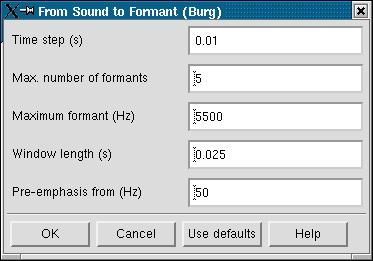
\includegraphics{/home/lennes/praat-opas/kuvat/formantti_burg_asetukset.jpg}


\caption{Formanttianalyysin asetusten määritteleminen.}
\end{figure}



\subsection{\label{sub:Tracking}Tracking }

Jos kaipaat yhtenäisiä ja johdonmukaisen näköisiä formanttikäyriä,
laske ensin edellämainitulla tavalla 2 Formant-objekti ja valitse
se objektilistasta. Paina sitten objektilistan oikeassa reunassa näkyvää
painiketta \textbf{Track\ldots{}} Tämä komento pyrkii löytämään jokaisesta
analyysi-ikkunasta (\emph{frame}) saman määrän formantteja ja esittämään
jokaiselle formantille suorimman mahdollisen \char`\"{}polun\char`\"{}
peräkkäisten ikkunoiden välillä. Jotta saisit esille esim. 3 formanttipolkua,
pitää Formant-objektin jokaisessa analyysi-ikkunassa olla ainakin
kolme formanttiehdokasta (ts. kannattaa laskea alkuperäinen formanttiobjekti
esim. 5 formantilla ja käyttää sitten \textbf{Track}-komentoa).


\subsection{Lisätietoa formanttianalyysista}

Kannattaa lukea Praatin sisäisestä manuaalista esim. tutoriaalisivu
\textbf{Source--filter~synthesis\index{Source--filter synthesis}}
(anna manuaalin hakusanaksi esim. \char`\"{}source-filter\char`\"{}),
jossa kuvataan melko helppotajuisesti puheen lähde-suodinteoria ja
neuvotaan käytännössä, miten Praatilla voi kokeilla puheen lähdeäänen
ja/tai ääntöväylän suodinfunktion laskemista puhenäytteestä. Sivu
on hyödyllinen varsinkin jos olet kiinnostunut Praatin puhesynteesiominaisuuksista.


\subsection{Formanttikuvien piirtäminen}

Tässä muutamia esimerkkejä Praatilla piirretyistä kuvista.

%
\begin{figure}
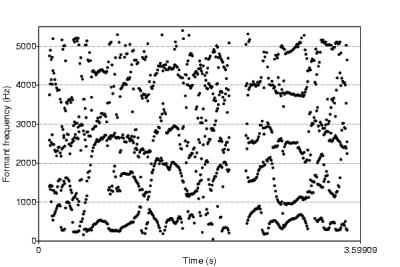
\includegraphics{/home/lennes/praat-opas/kuvat/formant_speckle.jpg}


\caption{Valitse Formant-objekti ja paina \textbf{Draw: Speckle\ldots{}}}
\end{figure}


\textbf{}%
\begin{figure}
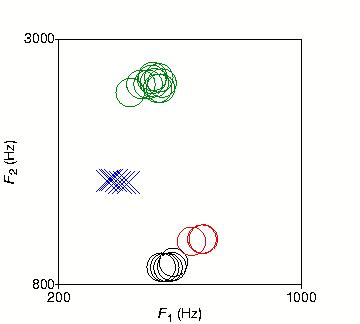
\includegraphics{/home/lennes/praat-opas/kuvat/formanttikarttaesim.jpg}


\caption{Valitse Formant-objekti ja paina \textbf{Draw: Scatter plot\ldots{}}
\protect \\
Esim. skriptaamalla voi myös lisätä kyseisen vokaalin nimen kunkin
ympyrän sisälle.}
\end{figure}



\subsection{F1/F2-formanttikartan piirtäminen}

Perinteisen, kirjallisuudessa usein esiintyvän F1/F2-vokaalikartan\index{F1/F2-vokaalikartta}\index{formanttikartta}
saa piirrettyä, kun ensin on laskenut tutkittavasta vokaalista tms.
yhtenäisestä äänteestä Formant-objektin objektilistaan esim. Burg-analyysilla
(\ref{par:formantit-objektilistasta}). 

\begin{enumerate}
\item Valitse Formant-objekti ja käytä komentoa \textbf{Draw --- Scatter~plot
(reversed~axes)\index{Scatter plot (reversed axes)}...} 
\item Määritä esiin tulevassa lomakkeessa F1:n arvot sijoitettavaksi pystyakselille
(\textbf{Vertical formant number:} 1)\textbf{\index{Vertical formant number}}
sekä sopivat F1:n ala- ja ylärajat kohtaan \emph{Vertical~minimum\index{Vertical minimum}}
ja \emph{Vertical~maximum}\textbf{\index{Vertical maximum}.} Määritä
F2 vastaavasti vaaka-akselille kirjoittamalla numero 2 kohtaan \emph{Horizontal
formant number\index{Horizontal formant number}} sekä antamalla ylä-
ja alarajat. F1:n ja F2:n rajat kannattaa valita niin, että ne juuri
ja juuri kattavat kaikkien vokaalilaatujen alueen kyseisellä puhujalla,
jolloin eri vokaalien pitäisi asettua erilleen ja helposti tulkittaviin
kohtiin kartalla. Piirrettävän merkin muodon ja koon voi valita piirtolomakkeen
alaosasta (\emph{Mark~size\index{Mark size}} ja \emph{Mark~string}\index{Mark string}).
Piirtoväriä voit vaihtaa vielä ennen lomakkeen hyväksymistä piirtoikkunan
\textbf{Pen}-valikosta. Muista myös valita piirtoikkunasta sopivan
kokoinen ja muotoinen alue, johon formanttikartta skaalautuu haluamallasi
tavalla (ks. \ref{sec:Kuvien-luominen}).
\item Paina \textbf{OK}. Tuloksena pitäisi olla vokaalikartta, jossa kummankin
formantin minimi on oikeassa ylänurkassa ts. kuvan pitäisi suunnilleen
vastata kirjallisuudessa näkyviä karttoja. Jos Formant-objekti on
laskettu niin pitkästä ääninäytteestä, että siihen on mahtunut useita
laskentaikkunoita, jokaisesta näistä piirtyy kuvaan yksi formanttipiste
tai -pallero. Tästä on iloa, jos piirrät formanttikartan esim. diftongista,
jolloin formanttien liike vokaalin aikana näkyy.
\item Voit piirtää samaan kuvaan päällekkäin muitakin Formant-objekteja.
Koska eri puhujien ''vokaaliavaruudet'' ovat hieman eri kokoisia
jo fysiologisista eroista johtuen, on yleensä järkevää piirtää vain
yhden puhujan formantteja samaan kuvaan.
\item Formanttikartan voi tallentaa kuvatiedostoon (\ref{sub:Kuvien-tallentaminen}).
\end{enumerate}

\subsection{Formanttianalyysin virhelähteet }

Formanttianalyysi perustuu teoreettiseen \label{l=E4hde-suodinteoria}malliin,
jonka mukaan akustinen puhesignaali muodostuu lähdeäänestä\index{l\"ahde-suodinteoria}
(esimerkiksi kurkunpään tuottama \char`\"{}surina\char`\"{}) ja ääntöväylän
suodinominaisuuksista (esimerkiksi formantit). Jos mitattavaan puheääneen
on päässyt vaikuttamaan jokin muu tekijä (esim. huonetila, muut puhujat
tai jokin äänitystekninen häiriö), saatat saada vääristyneitä mittaustuloksia.

\label{Formanttianalyysin-tulkinta}Formanttianalyysi vaatii aina
jonkin verran tulkintaa\index{formanttianalyysin tulkinta}: tutkija
olettaa formanttien löytyvän \char`\"{}sieltä mistä niiden pitäisi
löytyä\char`\"{}. Tutkijoiden käyttämät referenssiarvot perustuvat
lukuisiin tutkimuksiin, joissa yleensä selkeästi äännettyjen vokaalien
formantteja on mitattu tietyillä parametreilla kontrolloiduista aineistoista,
tai kaavamaiseen malliin \char`\"{}keskimääräisen\char`\"{} ääntöväylän
rakenteesta. Formanttilaskennan tuloksia ei saa pitää yksinomaan objektiivisina
lukuina, vaan ne on suhteutettava kyseiseen puhujaan, äänneympäristöön,
analyysiparametreihin ja äänitteen laatuun. Monet kontekstuaaliset
tekijät saattavat muuttaa formanttien taajuuksia ja kaistanleveyksiä,
ja jotkut puheen piirteet (esim. nasaalisuus) saattavat vaikeuttaa
formanttien tulkintaa. Puhujat ovat myös aina yksilöitä, eikä formanttiarvojen
pidäkään osua kaikilla samoille taajuuksille.

Formantteja kannattaa luonnollisesti mitata vain kohdista, joissa
ei ole usean puhujan päällekkäispuhuntaa. Näin varmistat, ettei toisten
puhujien ääni sekoita analyysia, sillä formanttianalyysi ei pysty
erottamaan eri äänilähteitä toisistaan. Myös muu taustahäly tai äänitystilan
voimakas jälkikaiku voivat periaatteessa aiheuttaa virheellisiä tuloksia.

Tavanomaiset formanttianalyysin asetukset sopivat parhaiten soinnillisiin
äänteisiin, etenkin vokaaleihin. Formantteja sinänsä on tietenkin
kaikissa äänteissä, mutta automaattisen formanttianalyysin parametrien
antaminen ja tulosten tulkinta on soinnittomilla äänteillä vaikeampaa,
joskus järjetöntäkin. Ei myöskään kannata käyttää \textbf{Track\ldots{}}-komentoa
kohdissa, joissa on esim. konsonantin ja vokaalin välinen siirtymä,
koska niissä löydettyjen formanttien lukumäärä saattaa äkisti muuttua,
jolloin järkevien \char`\"{}formanttipolkujen\char`\"{} löytäminen
on mahdotonta.

Kun formantit esiintyvät lähekkäin, kuten esim. F2 ja F3 {[}y{]}-vokaalissa
tai F1 ja F2 {[}u{]}:ssa tai {[}o{]}:ssa, on vaarana, että formanttianalyysi
tulkitsee vierekkäiset formantit samaksi yhtenäiseksi huipuksi. Näin
käy usein, jos tavanomaista viittä formanttia etsitään liian suurelta
taajuuskaistalta, esimerkiksi jos olet antanut matalaääniselle miespuhujalle
liian suuren yläraja-arvon kohdassa \emph{Maximum formant}.

Laskennallisesti tavallinen syy \label{formanttien-yhteensulautuminen}formanttien\index{formanttien yhteensulautuminen}
\char`\"{}yhtymiselle\char`\"{} tai \char`\"{}heittelehtimiselle\char`\"{}
on, ettei LPC-analyysissa ole käytetty riittävää määrää spektrikertoimia
(tämä lukuhan on suhteessa etsittävien formanttihuippujen määrään).
Riittävä määrä on vähintään signaalin näytteenottotaajuus hertseinä
jaettuna tuhannella (esim. 16 kHz signaalille 16). Praatin Burg-formanttianalyysi
näytteistää signaalin automaattisesti ensin näytetaajuuteen, joka
on kaksi kertaa \emph{Maximum formant}, ja jos (2 {*} Max. number
of formants) on tähän taajuuteen sopivassa suhteessa, kertoimia lasketaan
automaattisesti riittävä määrä ja analyysin pitäisi onnistua kohtalaisesti.
Sinun on kuitenkin otettava vielä tarkemmin huomioon oikea kerrointen
määrä, mikäli et käytä Praatin formanttianalyysia suoraan vaan teet
erikseen LPC-analyysin Sound-objektista. Silloin sinun on joko itse
näytteistettävä signaali uudestaan sopivaan näytetaajuuteen ennen
LPC-analyysia, tai annettava LPC:lle riittävä kertaluku (prediction
order), esim. 16 kHz ääninäytteelle 16. 


\chapter{\label{sec:Kuvien-luominen}Kuvien luominen}

\index{Picture-ikkuna}\index{piirtoikkuna}\index{piirtäminen}Praat-ohjelmalla
voi tarkastella ja tuottaa äänestä akustisia kuvauksia kahdella tavalla.
Siinä vaiheessa, kun aineistoon tutustutaan tai sitä nimikoidaan (ks.
\ref{sec:Nimikointi}), akustisia kuvantamismenetelmiä käytetään tavallisesti
editori-ikkunoiden, esimerkiksi äänieditorin (\ref{sec:Aanieditori-(Sound-editor)})
tai nimikointi-ikkunan (TextGrid-editorin, \ref{sub:TextGridin-tallennus})
kautta. Editori-ikkunoissa voi tehdä myös alustavia mittauksia erilaisista
analyysikuvista. Mikäli sen sijaan halutaan piirtää analyyseista laadukkaita
kuvia, jotka voidaan siirtää esimerkiksi tekstinkäsittelydokumenttiin,
on kyseinen analyysi ensin erikseen laskettava objektilistaan (ks.
\ref{sec:Akustinen-analyysi}). Piirtäminen Praat-ohjelman piirtoikkunaan
tapahtuu nimittäin aina jonkin objektilistassa olevan objektin pohjalta.


\section{Kuvan piirtäminen}

\begin{enumerate}
\item Valitse objekti-ikkunasta se objekti/objektit, josta haluat piirtää
kuvan. Jos haluat piirtää analyysikuvan, jota vastaavaa objektia ei
vielä listassa ole, valitse ensin ääniobjekti ja laske siitä haluamasi
analyysiobjekti (ks. \ref{sec:Akustinen-analyysi})
\item Valitse hiirellä \emph{piirtoikkunasta} (\emph{Picture}) haluamasi
kokoinen ja muotoinen suorakaide (\emph{Viewport}\index{Viewport}),
johon kuva piirretään. 
\item Muuta tarvittaessa piirrettävän kuvan piirtoväriä (piirtoikkunan valikosta
\textbf{Pen}) ja/tai tekstin kirjasintyyppiä ja -kokoa (piirtoikkunan
valikosta \textbf{Font}). Tämä valinta vaikuttaa vasta seuraavan kuvan
ominaisuuksiin, ei piirtoikkunan aikaisempaan sisältöön.
\item Valitse objekti-ikkunasta se objekti, josta haluat piirtää kuvan.
Valitse sitten dynaamisesta valikosta joko \textbf{Draw}- tai \textbf{Paint}-painikkeen
alta sopiva piirtokomento (Paint-komento näkyy Draw-komennon sijaan
esimerkiksi spektrogrammiobjektin ollessa valittuna). Näkyviin tulee
lomake, jossa kysytään joitakin piirrettävään kuvaan liittyviä tietoja. 

\begin{itemize}
\item \emph{Garnish}-kohdassa oleva rasti tarkoittaa, että kuvan ympärille
piirretään automaattisesti laatikko ja merkitään vaaka- ja pystyakseleille
oletusarvoiset nimet ja asteikot. Jos jostakin syystä haluat esimerkiksi
piirtää päällekkäin kuvia eri objekteista tai haluat määritellä akseleiden
otsikot ja numerot itse, ota \emph{Garnish}-ruksi pois.
\end{itemize}
\item Paina \textbf{OK}, jolloin kuva piirtyy piirtoikkunasta valitun alueen
sisään. Kuva skaalautuu automaattisesti alueen muotoiseksi.
\end{enumerate}

\section{\label{sub:Kuvien-tallentaminen}Kuvien tallentaminen}

Ennen kuin tallennat tai siirrät kuvaa Praatin piirtoikkunasta, valitse
varmuuden vuoksi se osa piirtoalueesta, jonka haluat tallentaa tai
siirtää. 

Praat-ohjelman piirtoikkunaan piirretyn kuvan voi joko

\begin{enumerate}
\item \emph{kopioida leikepöydälle\index{kuvan siirto leikepöydälle}} komennolla
\textbf{Copy to clipboard} (toimii Praatin Windows- ja Macintosh-versioissa)
\emph{}ja sen jälkeen liittää vaikkapa tekstinkäsittelydokumenttiin
ko. ohjelman \textbf{Edit}- valikon \textbf{Paste}-komennolla. Huom.
kuva ei tallennu minnekään ennen kuin tallennat toisessa ohjelmassa
käsittelemäsi dokumentin!
\item \emph{tallentaa} Praat-kuvana\index{Praat-kuvatiedosto}, jota ei
voi avata millään muulla ohjelmalla, käyttämällä komentoa \textbf{File:
Write to praat picture file...} Praat-kuvatiedostoja kannattaa käyttää,
jos haluat jatkossa yhdistää tiettyyn kuvaan uusia kuvia tai jatkaa
sen piirtämistä Praatilla. Praat-kuvatiedostojen oletusarvoinen tiedostopääte
on \emph{.prapic}
\item \emph{tallentaa} \label{enu:EPS-grafiikka}EPS-muotoisena kuvatiedostona
komennolla \textbf{File: Write to EPS file...} EPS-kuvatiedostojen
nimissä kannattaa käyttää tiedostopäätettä \emph{.eps}
\end{enumerate}
\emph{EPS\index{EPS}} eli \emph{Encapsulated Postscript\index{Encapsulated Postscript}}
on kuvaformaatti, jota kannattaa aina käyttää painatettavaksi tarkoitetussa
materiaalissa. EPS on nimittäin skaalautuvaa vektorigrafiikkaa toisin
kuin esimerkiksi piirtoikkunasta copy-paste-menetelmällä siirretyt
bittikarttakuvat, jotka ovat laadultaan heikompia ja muuttuvat jälkeenpäin
venytettäessä rakeisiksi. PostScript on oikeastaan yleinen grafiikan
ja tekstin kuvauskieli, jota suunnilleen kaikki nykyiset lasertulostimet
käyttävät tulostettavan materiaalin käsittelyyn. EPS-grafiikka takaa
siis myös, että aineisto tulostuu hyvälaatuisena.


\section{\label{sub:Kuvatiedostojen-avaaminen-Praatin}Kuvatiedostojen avaaminen
Praatin piirtoikkunaan}

Praat-ohjelmalla tallennetuista tai muualle siirretyistä kuvista voidaan
Praatilla avata ainoastaan \emph{praat picture}-tiedostot. Valitse
piirtoikkunassa komento \textbf{File: Read from praat picture file...} 


\section{\label{sub:Kuvatiedostojen-avaaminen-muilla}Kuvatiedostojen avaaminen
muilla ohjelmilla}

Praat-ohjelmalla tallennettuihin EPS-kuvatiedostoihin ei valitettavasti
erikseen tallennu ns. esikatselukuvaa. Tämä tarkoittaa, että kun liität
Praatilla tekemäsi EPS-tiedoston esimerkiksi Word-dokumenttiin, kuvan
kohdalla näkyy vain laatikko, jonka päällä on ruksi. Kun tulostat
Word-dokumentin paperille, kuva kuitenkin näkyy vastaavassa kohdassa. 

Erityisillä grafiikkaohjelmilla EPS-kuviinkin voi luoda esikatselukuvan,
jos sellaista tarvitsee. Kaikki kuvankäsittelyohjelmat eivät välttämättä
tue EPS-grafiikkaa, mutta sellaiset ammattikäyttöön tarkoitetut piirto-ohjelmat
kuin Adobe Illustrator tai Macromedia Freehand kylläkin. 

Varmin tapa saada EPS-kuvatiedosto auki on käyttää erityistä ohjelmaa,
joka on tarkoitettu PostScript-dokumenttien käsittelyyn ja näyttämiseen.
Tällainen ilmainen ohjelmistopaketti on \emph{Ghostscript} ja sen
pariksi tarkoitettu PS-dokumenttien katseluohjelma nimeltä \emph{Ghostview}
(tai \emph{GSview}), jotka voi ladata ilmaiseksi verkosta, \url{http://www.cs.wisc.edu/\~ghost/}.
Nämä ohjelmat kannattaa Windows-käyttäjän asentaa koneelleen, sillä
niillä on Praatilla tehtyjen kuvien katselun ja muuntamisen lisäksi
muutakin käyttöä. Unix- ja Linux-käyttäjien ei yleensä tarvitse olla
huolissaan PostScript-dokumenttien avaamisesta, sillä unix-tyyppisissä
käyttöjärjestelmissä on yleensä valmiina postscript-tuki.


\chapter{\label{cha:Skriptaus}Skriptaus}


\section{\label{sec:Mika-on-skripti?}Mikä on skripti?}

Skripti\index{skripti} on eräänlainen tietokoneohjelma, jonka on
tarkoitus olla helposti omaksuttavissa ja suhteellisen helppolukuinen.

Skriptikielen komennot on yleensä suunniteltu johonkin erityiseen
tarkoitukseen ja toimivat vain tietyssä rajatussa ympäristössä. Esimerkiksi
Praat-skriptillä ei tee mitään, jollei koneeseen ole asennettu Praat-ohjelmaa,
jolla skriptin voisi suorittaa.

Itse \textbf{skripti on tavallinen tekstitiedosto}, jossa on yksi
tai useampia rivejä. Kullakin rivillä on yksi komentolause.

Monet Praat-skriptien komennoista ovat aivan samannäköisiä kuin Praatissa
näkyvät valikkokomennotkin (ks. \ref{sec:Historiatoiminto}).

Skriptin voit siis kirjoittaa ja avata uudelleen muokattavaksi millä
tahansa tekstieditorilla\index{tekstieditori}

%
\footnote{Unix/Linux-koneissa vaihtoehtoja riittää: esim. \emph{emacs} tai \emph{pico}.
Vanhemmissa Macintosheissa hyvä valinta on esim. \emph{BBEdit} (josta
pitäisi löytyä ilmaisia versioita). Windows-koneissa voit käyttää
esimerkiksi \emph{WordPad}ia tai jotakin ilmaista verkosta löytyvää
tekstieditoria (itse kokeilin esim. \emph{NoteTab Light} -nimistä
ohjelmaa). %
} (tai tekstinkäsittelyohjelmalla, jos tallennat työn tuloksen tavallisena
tekstitiedostona). Praatissa ei ole merkitystä sillä, mikä on skriptitiedoston
tiedostopääte.

Myös Praatissa on sisäänrakennettuna oma yksinkertainen tekstieditori\index{tekstieditori},
jolla voit luoda ja muokata skriptejä, mutta siinä ei ole juuri mitään
kirjoitustyötä helpottavia hienouksia (edes rivinumerointia), mikä
saattaa ärsyttää pitemmälle ehtinyttä skriptaajaa.

\begin{comment}
Edistyneemmille käyttäjille vinkkinä: Praatin skriptikielellä voi
tehdä paljon kaikenlaista. Mitä monimutkaisempia toimintoja huomaa
skripteihin kirjoittavansa, sitä tarkemmin pitäisi kuitenkin miettiä,
löytyisikö tarkoitukseen paremmin sopivia skriptaus- tai ohjelmointikieliä.
(Oppaan kirjoitushetkellä kirjoittaja tekee melkein kaiken Praatilla,
koska ei osaa muutakaan... ;-D)

Eri kielillä tehtyjä palikoita voi myös yhdistellä kekseliäästi. Esim.
Perl -skriptit saattavat olla joihinkin tarkoituksiin kätevämpiä,
jollei Praatin signaalinkäsittelytoimintoja tarvita - ja jos osaa
Perliä. Ehkä kannattaa kokeilla PraatJavaa , jos Java-ohjelmointi
on lähellä sydäntä. Praat sinänsä on kirjoitettu C:llä, joten C:n
taitaja voi kehitellä Praatin lähdekoodiin lisätoimintoja ja kääntää
vaikka itselleen oman Praat-version.
\end{comment}

\section{\label{sec:Mita-hyotya-skriptaamisesta}Miksi skriptejä käytetään? }

Skripteillä voi selviytyä nopeammin, johdonmukaisemmin ja vähemmin
virhein toistuvista tehtävistä, jotka \char`\"{}käsin\char`\"{} tehtynä
olisivat aikaavieviä, tylsiä ja virhealttiita. Yksinkertainenkin skripti
saattaa helpottaa elämää huomattavasti. Lisäksi skripteillä voi usein
korvata toimintoja, jotka Praatista (toistaiseksi) sattuvat puuttumaan.
Skriptien kirjoittamiseen kannattaa siis uhrata hieman aikaa - varsinkin
jos tietää, että edessä on oikea \char`\"{}liukuhihnaprojekti\char`\"{}!


\section{Praat-skriptin luominen ja muokkaus}

\begin{itemize}
\item Jos haluat luoda uuden skriptin\index{skriptin luominen} Praatilla,
valitse objektilistan \textbf{Control}-valikosta (tai jonkin editori-ikkunan
\textbf{File}-valikosta) \textbf{New~script}. Skriptieditori\index{skriptieditori}
aukeaa. Kirjoita skriptirivit tavalliseen tapaan ja tallenna\index{skriptin tallentaminen}
skripti \textbf{File}-valikosta komennolla \textbf{Save}.
\item Kun haluat avata\index{skriptin avaaminen} jo aikaisemmin tallennetun
skriptin Praatissa, valitse 

\begin{itemize}
\item objektilistan \textbf{Control}-valikosta \textbf{Open~script\ldots{} }
\item tai jonkin editori-ikkunan \textbf{File}-valikosta \textbf{Open~editor~script\ldots{}}
\end{itemize}
\noindent Tässä vaiheessa on huomioitava, kumpaa kautta skripti on
tarkoitettu avattavaksi: editoriskriptit eivät välttämättä toimi,
jos ne avataan objektilistan valikosta ja päinvastoin.

\end{itemize}

\section{\label{sec:Historiatoiminto}Skriptauksen opettelu historiatoiminnon
avulla}

Historiatoiminto\index{historiatoiminto} on helpoin tapa aloittaa
skriptaus Praatissa. Historiaominaisuus muistuttaa hieman esimerkiksi
Microsoft Wordin makroja, joihin voi ensin tallettaa erilaisia toimenpidesarjoja
ja toistaa niitä sitten yhä uudelleen.

\begin{itemize}
\item Avaa skripti tai luo uusi Praatin omaan tekstieditoriin (ks. edellinen
kohta). 
\item Kokeile skripti-ikkunan \textbf{Edit}-valikon komentoa \textbf{Paste~history}\index{Paste history}.
Praat kirjoittaa skriptikielellä kaikki ne toiminnot, joita olet suorittanut
siitä saakka kun Praatin avasit.
\item \textbf{Edit}-valikon komento \textbf{Clear~history} tyhjentää historian
ja aloittaa sen keräämisen alusta, jolloin voit tallettaa skriptiin
vain muutaman viimeisimmän komennon. Historian avulla on helppo \char`\"{}luntata\char`\"{},
miten jokin asia Praatin skriptikielessä tehdään.
\end{itemize}
Huom. Kaikki Praatissa näkyvät valikkokomennot ja painikkeet ovat
samalla skriptikielen komentoja! Voit siis myös \char`\"{}luntata\char`\"{}
komentoja katsomalla niiden tarkan sanamuodon suoraan valikoista.
Jos esimerkiksi analyysin tekemiseen kysytään käyttäjältä tietoja:
esim. Pitch-analyysissa '\emph{time step}', '\emph{minimum pitch}'
ja '\emph{maximum pitch}', nämä tiedot pitää skriptatessa antaa samassa
järjestyksessä varsinaisen \textbf{To~Pitch...}-komennon perään välilyönneillä
erotettuna. Esimerkiksi komento

\textsf{To~Pitch...~0.01~75~400}

laskee Pitch-objektin parametreillä 0.01 sekuntia, 75 Hz ja 400 Hz.

Historiatoiminto on kätevä, mutta se ei anna käyttöösi kaikkia skriptikielen
\char`\"{}ohjelmointiteknisiä\char`\"{} mahdollisuuksia. Et esimerkiksi
voi tuottaa historiatoiminnolla muuttujia, käsitellä merkkijonoja
tai tehdä silmukkaa l. toistaa samaa komentosarjaa vaihtelevilla parametreilla
ilman, että tekisit kaiken ensin kohta kohdalta käsin. Historia auttaa
siis alkuun ja antaa vinkkejä skriptin eri osia varten. Mitä monimutkaisempi
toimintosarja, sitä enemmän joudut luultavasti itse miettimään. 

Katso siis lisäohjeita Praatin sisäisestä manuaalista , kohdasta Scripting
tutorial! 


\section{\label{sec:Miten-skripti-suoritetaan}Skriptin suorittaminen (ajaminen) }

Jos olet löytänyt skriptin verkosta, lataa se ensin omalle koneellesi
ja tallenna sopivaan paikkaan.

\begin{enumerate}
\item Jotta voit suorittaa (ajaa) skriptin, sinun on avattava se Praatin
omaan skriptieditoriin\index{skriptieditori} vähintään kerran.

\begin{itemize}
\item Skripti avataan objektilistasta käsin valitsemalla \textbf{Control}-valikosta
\textbf{Open script... }
\item Erilaisista editori-ikkunoistakin voit skriptin avata. Tällöin \textbf{Open
script...}-komento löytyy kyseisen editorin \textbf{File}-valikosta.
\end{itemize}
\item Kun skripti-ikkuna on näkyvissä, voit suorittaa skriptin valitsemalla
\textbf{Run\ldots{}~->~Run}.
\end{enumerate}
Huom. Jos luot usein käyttämällesi Praat-skriptille oman valikkokomennon
tai painikkeen (ks. alla), sinun ei tarvitse myöhemmin enää avata
skriptiä Praatissa kyseisellä koneella, kunhan säilytät skriptitiedoston
samannimisenä samassa paikassa.


\section{\label{sec:Valikkokomennot-ja-painikkeet}Valikkokomentojen ja painikkeiden
luominen skripteille }


\subsection{\label{sub:Valikkokomennon-luonti-skriptille}Valikkokomennon luonti
skriptille (fixed menu)}

\begin{enumerate}
\item Avaa skripti sellaisen Praatin ikkunan sisältä, johon valikkokomennon\index{valikkokomennon luominen}
tai painikkeen pitäisi liittyä.

\begin{itemize}
\item Jos haluat, että komento tulee objektilistan tai piirtoikkunan johonkin
valikkoon, valitse objektilistan \textbf{Control}-valikosta \textbf{Open
script...} Valitse sitten \textbf{File}-valikosta \textbf{Add to fixed
menu...}
\item Jos taas haluat komennon esim. TextGrid-editori-ikkunan valikkoon,
avaa ensin TextGrid-editori mille tahansa TextGrid- ja ääniobjektille
ja valitse editorin \textbf{File}- valikosta \textbf{Open script...}
Valitse sitten \textbf{File}-valikosta \textbf{Add to menu...}
\end{itemize}
\item Kirjoita, mihin valikkoon (\emph{Menu}) uuden komennon haluat ja mikä
komennon teksti (\emph{Command}) on. Jos avasit skriptin jostakin
editori-ikkunasta, komento tulee näkyviin valikkoon vasta, kun seuraavan
kerran avaat uuden editori-ikkunan.
\end{enumerate}

\subsection{\label{sub:Painikkeen-luonti-skriptille}Painikkeen luonti skriptille
(dynamic menu)}

Painikkeen\index{painikkeen luominen} voit luoda vain objektilistaan.

\begin{enumerate}
\item Valitse objektilistan \textbf{Control}-valikosta \textbf{Open script...}
Valitse sitten skripti-ikkunan File-valikosta Add to dynamic menu... 
\item Kirjoita kohtaan \emph{Class 1} se objektityyppi (esim. Sound tai
TextGrid), jonka on oltava objektilistassa valittuna, jotta painike
olisi näkyvissä. 
\item Kirjoita kohtaan \emph{Number 1}, montako \emph{Class 1}-tyyppistä
objektia on vähintään oltava valittuna, jotta painike näkyisi. Jos
lukumäärällä ei ole väliä, jätä tähän kohtaan 0.
\item Kirjoita kohtaan \emph{Command} se teksti, jonka haluat näkyvän painikkeessa.
\item Tarkista, että kohdassa \emph{Script file} on oikea tiedostopolku
skriptiin. 
\item Paina \emph{OK}.
\end{enumerate}

\subsection{\label{sub:Valikkokomennon-poistaminen}Valikkokomennon tai painikkeen
poistaminen}

\begin{enumerate}
\item Valikkokomennon\index{Valikkokomennon poistaminen tai k\"atkeminen}
tai painikkeen voit poistaa objektilistan \textbf{Control}-valikon
komennolla \textbf{Preferences...:} \textbf{Buttons...}
\item Näkyviin tulee ikkuna, jossa on luettelot kaikista Praatin valikkokomennoista
ja painikkeista. Ikkunan yläreunasta voit valita, näytetäänkö esim.
objektilistan vai piirtoikkunan valikot vai esim. kaikki painikkeet
A:sta M:ään. 
\item Praatin sisäänrakennettujen komentojen kohdalla voit valita, onko
komento näkyvissä (\emph{shown}) vain käyttäjältä piilossa (\emph{hidden}).
\item Itse lisäämiesi komentojen ja painikkeiden kohdalla lukee \emph{ADDED},
ja kun klikkaat kyseistä kohtaa, teksti muuttuu muotoon \emph{REMOVED}
ja komento häviää Praatista. Skripti tietenkin pysyy tallella ja voit
uudestaan käyttää sitä Praatissa milloin tahansa.
\end{enumerate}

\section{Mitä vaaroja skriptien käyttämisessä voi olla?}

\begin{itemize}
\item Praat-skriptikin\index{skriptauksen huonot puolet} voi olla mahdollinen
tietoturvariski. Käytä vain skriptejä, jotka saat luotettavasta lähteestä
ja joiden toiminnan varmasti tunnet. Älä myöskään itse kirjoita skriptejä,
jotka esim. poistavat tiedostoja käyttäjältä kysymättä.
\item Esimerkiksi erilaisia akustisia analyyseja on hyvin helppo automatisoida
skriptaamalla. Jollet kuitenkaan tunne analyysien käyttöaluetta ja
analyysiparametrien toimintaa, saatat tietämättäsi tuottaa järjettömiä
tuloksia. Praat ei tarkista, miten fiksuja tai luotettavia mittauksesi
ovat, kunhan skriptin syntaksi on korrekti!
\item Testaa aina skriptiäsi ensin pienellä aineistolla ja tutki käsin,
ovatko skriptin tuottamat mittaustulokset oikeita. Kokeneellekin voi
sattua pikku kirjoitusvirheitä\ldots{}
\end{itemize}
\listoffigures


\printindex{}

\bibliographystyle{plain}
\cleardoublepage\addcontentsline{toc}{chapter}{\bibname}\bibliography{/home/lennes/bib/ref}

\end{document}
